% !TEX program = xelatex
\documentclass[UTF8,a4paper,11pt]{ctexart}

\usepackage[a4paper,margin=2.0cm,headheight=14pt]{geometry}
\usepackage{amsmath,amssymb,booktabs,longtable,array,tabularx}
\usepackage{caption}
\usepackage{graphicx}
\usepackage{pdflscape}
\usepackage{xcolor}
\usepackage{xurl}
\usepackage{hyperref}

\definecolor{pyblue}{RGB}{36,91,163}
\definecolor{qudared}{RGB}{190,65,55}
\hypersetup{
  colorlinks=true,
  linkcolor=pyblue,
  urlcolor=pyblue,
  pdftitle={PyQCU 与 QUDA MultiGrid 对比测试报告（绝对耗时修订版）}
}
\graphicspath{
  {../data/report_multigrid_comprehensive_20260929/report/}
  {../data/report_multigrid_comprehensive_20260928/final_protocol/report/}
  {../data/report_multigrid_comprehensive_20260928/final_protocol/}
}
\newcolumntype{L}[1]{>{\raggedright\arraybackslash}p{#1}}
\newcolumntype{Y}{>{\raggedright\arraybackslash}X}
\newcommand{\code}[1]{\texttt{\detokenize{#1}}}
\setlength{\parindent}{2em}
\setlength{\parskip}{0.35em}
\emergencystretch=3em

\title{PyQCU 与 QUDA MultiGrid 对比测试报告\\绝对耗时修订版}
\author{PyQCU 测试记录}
\date{2026 年 9 月 29 日}

\begin{document}
\maketitle

\begin{abstract}
本报告是 2026-09-28 正式矩阵报告的派生修订版。所有性能事实继续使用
\code{git tag test27}（commit
\code{04382801c003353ecd1bc6b9bc10f6db750bf74d}）保存的原始
combined JSON、CSV 和 trace，不重新采样、不替换配置、不修改原始数据。
修订重点是展示层：保留时间比，同时给出 PyQCU 与 QUDA 的 steady
绝对秒数；把 66 个精确单元的散点、trace-off MG 分组耗时和
BiCGStab 参考耗时改成可直接读数的图；重排逐层阶段图并显式标出
QUDA 最后一个有效层及其最粗层 solve；最细层总览图例统一移到图表下方。

正式覆盖仍为 66 个 combined 精确单元和 132 条 side record，全部通过
配置哈希、输入 bundle、1 cold / 2 warmup / 5 steady、公平性和独立
full-operator 真残差门。双 P100 的
$16\times32\times32\times48$ c64 请求仍按原记录使用 $16^4$ 容量替代，
替代项不进入原始大格公平比较。
\end{abstract}

\tableofcontents

\section{数据口径与验收标准}

本版不改变正式测试协议。所有绝对耗时均直接来自 test27 的
\path{combined/*.json}：MG-2/3 取
\path{sides.<side>.timing.steady.median_seconds}，BiCGStab 参考取
\path{sides.<side>.reference_solver.steady.median_seconds}。逐层耗时取
\path{sides.<side>.mg_levels}，trace-on 用于阶段归因，trace-off 用于
正式性能结论。

\begin{table}[htbp]
\centering
\caption{固定测试与统计协议}
\small
\begin{tabularx}{\textwidth}{@{}L{0.25\textwidth}Y@{}}
\toprule
维度 & 取值 \\
\midrule
实现 & QUDA 1.1.0，PyQCU Strict CUDA/C++ \\
设备 & 单卡 Tesla V100-SXM2-32GB；双 Tesla P100-PCIE-16GB \\
c64 格点 & $8^3\times16$，$16^4$，$16\times32\times32\times48$ \\
c128 格点 & $8^3\times16$，$16^4$，$16\times16\times32\times32$ \\
trace & on，off \\
求解 & BiCGStab 参考，MG-2，MG-3 \\
phase & 1 cold，2 warmup，5 steady \\
中心值 & steady median；MAD 与原始样本保留在 side JSON \\
真残差门 & full periodic Wilson/Clover，相对残差 $<5\times10^{-6}$ \\
资源门 & 单 collector $\le570$ s；设备显存峰值 $<85\%$ \\
\bottomrule
\end{tabularx}
\end{table}

\begin{table}[htbp]
\centering
\caption{覆盖与公平性硬门禁}
\small
\begin{tabular}{@{}lrr@{}}
\toprule
项目 & 观察值 & 要求 \\
\midrule
combined 精确单元 & 66 & 66/66 通过 \\
side record & 132 & 132/132 通过 \\
1 cold / 2 warmup / 5 steady & 132/132 & 全部完整 \\
config hash 一致 & 66/66 & 全部一致 \\
input bundle 一致 & 66/66 & 全部一致 \\
full true residual 通过 & 66/66 & 全部 $<5\times10^{-6}$ \\
trace-on MG residual curve & 44/44 & 全部存在 \\
MG level row & 220/220 & 无缺失字段 \\
\bottomrule
\end{tabular}
\end{table}

\begin{figure}[htbp]
\centering
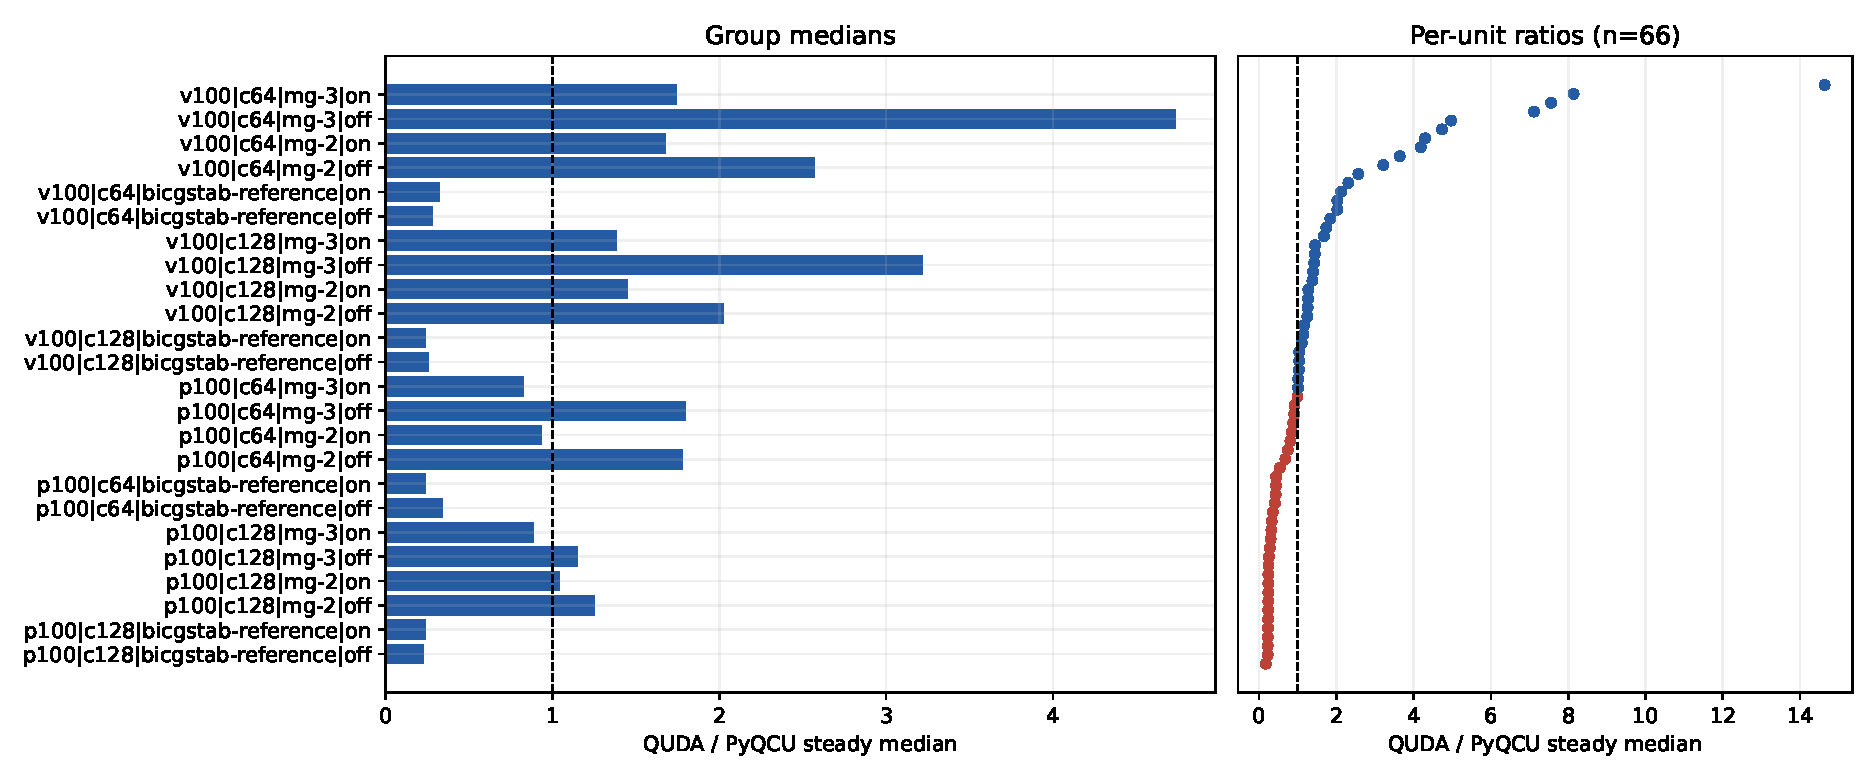
\includegraphics[width=0.98\linewidth,height=0.70\textheight,keepaspectratio]{overlap_matrix.pdf}
\caption{按设备、精度、求解器和 trace 模式分组的中位时间比。
$R=t_{\mathrm{QUDA,steady}}/t_{\mathrm{PyQCU,steady}}$，$R>1$
表示 QUDA 更慢、PyQCU 更快。}
\label{fig:overlap}
\end{figure}

请求矩阵共 72 个 combined 单元和 144 个 side-case。精确完成 66 个
combined 单元和 132 个 side-case；其余 6 个 combined 单元仅对应
双 P100 c64 大格容量替代。逐请求状态和替代映射分别见
\path{requested_matrix_status.csv} 与
\path{capacity_substitutions.csv}。

\section{构建与运行 provenance}

\begin{table}[htbp]
\centering
\caption{设备和二进制身份}
\small
\begin{tabularx}{\textwidth}{@{}L{0.17\textwidth}L{0.35\textwidth}Y@{}}
\toprule
设备 & 运行栈 & 二进制与架构 \\
\midrule
V100 & PyTorch 2.10.0+cu128；CUDA 12.8；PyQUDA 0.10.54 &
\path{cpp/cuda/qcu/libqcu.so}，SHA256
\code{81ec614211a50954...a670889}，\code{sm_70} cubin；
QUDA \code{quda-double-install}，\code{sm_70}，
QIO/QMP/MG-double/reconstruct 7 \\
P100 & PyTorch 2.7.1+cu118；CUDA 11.8；PyQUDA 0.10.54 &
\path{data/build/libqcu_arch/sm60/libqcu.so}，SHA256
\code{e29c1cf04a57ec3b...d0c20e1}，\code{sm_60} cubin；
QUDA \code{quda-sm60-install}，\code{sm_60}，
QIO/QMP/MG-double/reconstruct 7 \\
\bottomrule
\end{tabularx}
\end{table}

报表派生器记录 test27 commit、66 个 combined 输入路径及源 CSV 哈希，
见 \path{source_manifest.json}。其中 \path{units.csv} 的 SHA256 为
\code{8ab3e1e6...779177e4e}，\path{stages.csv} 的 SHA256 为
\code{61a7263b...1e928e36}。这些哈希用于确认修订版没有换用
2026-09-27 之前或其他轮次的数据。

\section{绝对耗时与时间比}

时间比定义为
\begin{equation}
  R = \frac{t_{\mathrm{QUDA,steady}}}
           {t_{\mathrm{PyQCU,steady}}}, \qquad R>1\text{ 有利于 PyQCU}.
\end{equation}
下表同时列出两侧绝对中位秒数。表内 \code{median} 是组内各单元
时间比的中位数，不是两个组中位秒数的比值；因此保留时间比和绝对耗时
可以独立核验。

\begin{longtable}{@{}lllrrrrr@{}}
\caption{分组绝对 steady 耗时与时间比（trace-on/off 分开统计）}\label{tab:group-times}\\
\toprule
设备 & 精度 & 求解 & trace & $n$ & PyQCU 中位 s & QUDA 中位 s & $R$ 中位 \\
\midrule
\endfirsthead
\toprule
设备 & 精度 & 求解 & trace & $n$ & PyQCU 中位 s & QUDA 中位 s & $R$ 中位 \\
\midrule
\endhead
P100 & c128 & BICGSTAB & off & 3 & 3.896 & 0.874 & 0.2284 \\
P100 & c128 & BICGSTAB & on & 3 & 3.767 & 0.899 & 0.2400 \\
P100 & c128 & MG-2 & off & 3 & 6.410 & 6.634 & 1.2502 \\
P100 & c128 & MG-2 & on & 3 & 8.686 & 7.052 & 1.0420 \\
P100 & c128 & MG-3 & off & 3 & 4.688 & 5.185 & 1.1517 \\
P100 & c128 & MG-3 & on & 3 & 8.364 & 5.713 & 0.8843 \\
P100 & c64 & BICGSTAB & off & 2 & 1.178 & 0.405 & 0.3416 \\
P100 & c64 & BICGSTAB & on & 2 & 1.694 & 0.403 & 0.2368 \\
P100 & c64 & MG-2 & off & 2 & 1.055 & 1.995 & 1.7773 \\
P100 & c64 & MG-2 & on & 2 & 2.450 & 2.166 & 0.9341 \\
P100 & c64 & MG-3 & off & 2 & 1.073 & 2.057 & 1.7944 \\
P100 & c64 & MG-3 & on & 2 & 2.894 & 2.263 & 0.8282 \\
V100 & c128 & BICGSTAB & off & 3 & 0.552 & 0.146 & 0.2580 \\
V100 & c128 & BICGSTAB & on & 3 & 0.650 & 0.146 & 0.2397 \\
V100 & c128 & MG-2 & off & 3 & 0.721 & 1.461 & 2.0269 \\
V100 & c128 & MG-2 & on & 3 & 1.085 & 1.575 & 1.4515 \\
V100 & c128 & MG-3 & off & 3 & 0.436 & 1.525 & 3.2174 \\
V100 & c128 & MG-3 & on & 3 & 1.173 & 1.621 & 1.3822 \\
V100 & c64 & BICGSTAB & off & 3 & 0.242 & 0.068 & 0.2818 \\
V100 & c64 & BICGSTAB & on & 3 & 0.250 & 0.084 & 0.3213 \\
V100 & c64 & MG-2 & off & 3 & 0.204 & 0.524 & 2.5717 \\
V100 & c64 & MG-2 & on & 3 & 0.383 & 0.644 & 1.6785 \\
V100 & c64 & MG-3 & off & 3 & 0.151 & 0.715 & 4.7366 \\
V100 & c64 & MG-3 & on & 3 & 0.528 & 0.921 & 1.7444 \\
\bottomrule
\end{longtable}


\begin{figure}[htbp]
\centering
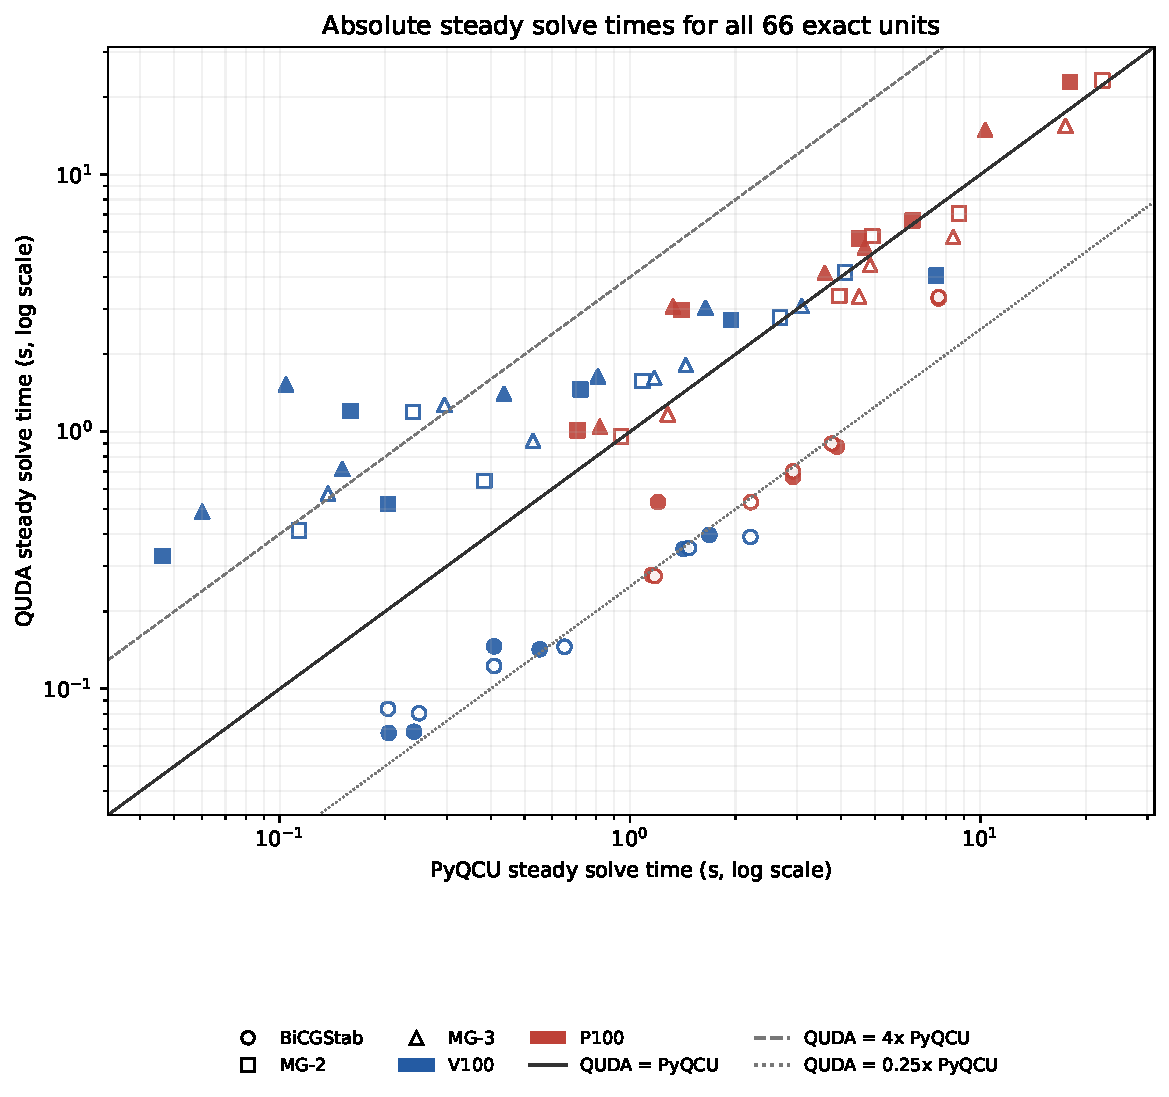
\includegraphics[width=0.93\linewidth,height=0.72\textheight,keepaspectratio]{mg_time_tradeoff.pdf}
\caption{66 个精确单元的 PyQCU 与 QUDA 绝对 steady 耗时。
横纵轴均为秒，实线为 $y=x$，虚线、点线分别对应
$y=4x$ 与 $y=0.25x$；空心标记为 trace-on，实心标记为 trace-off。}
\label{fig:time-tradeoff}
\end{figure}

\begin{figure}[htbp]
\centering
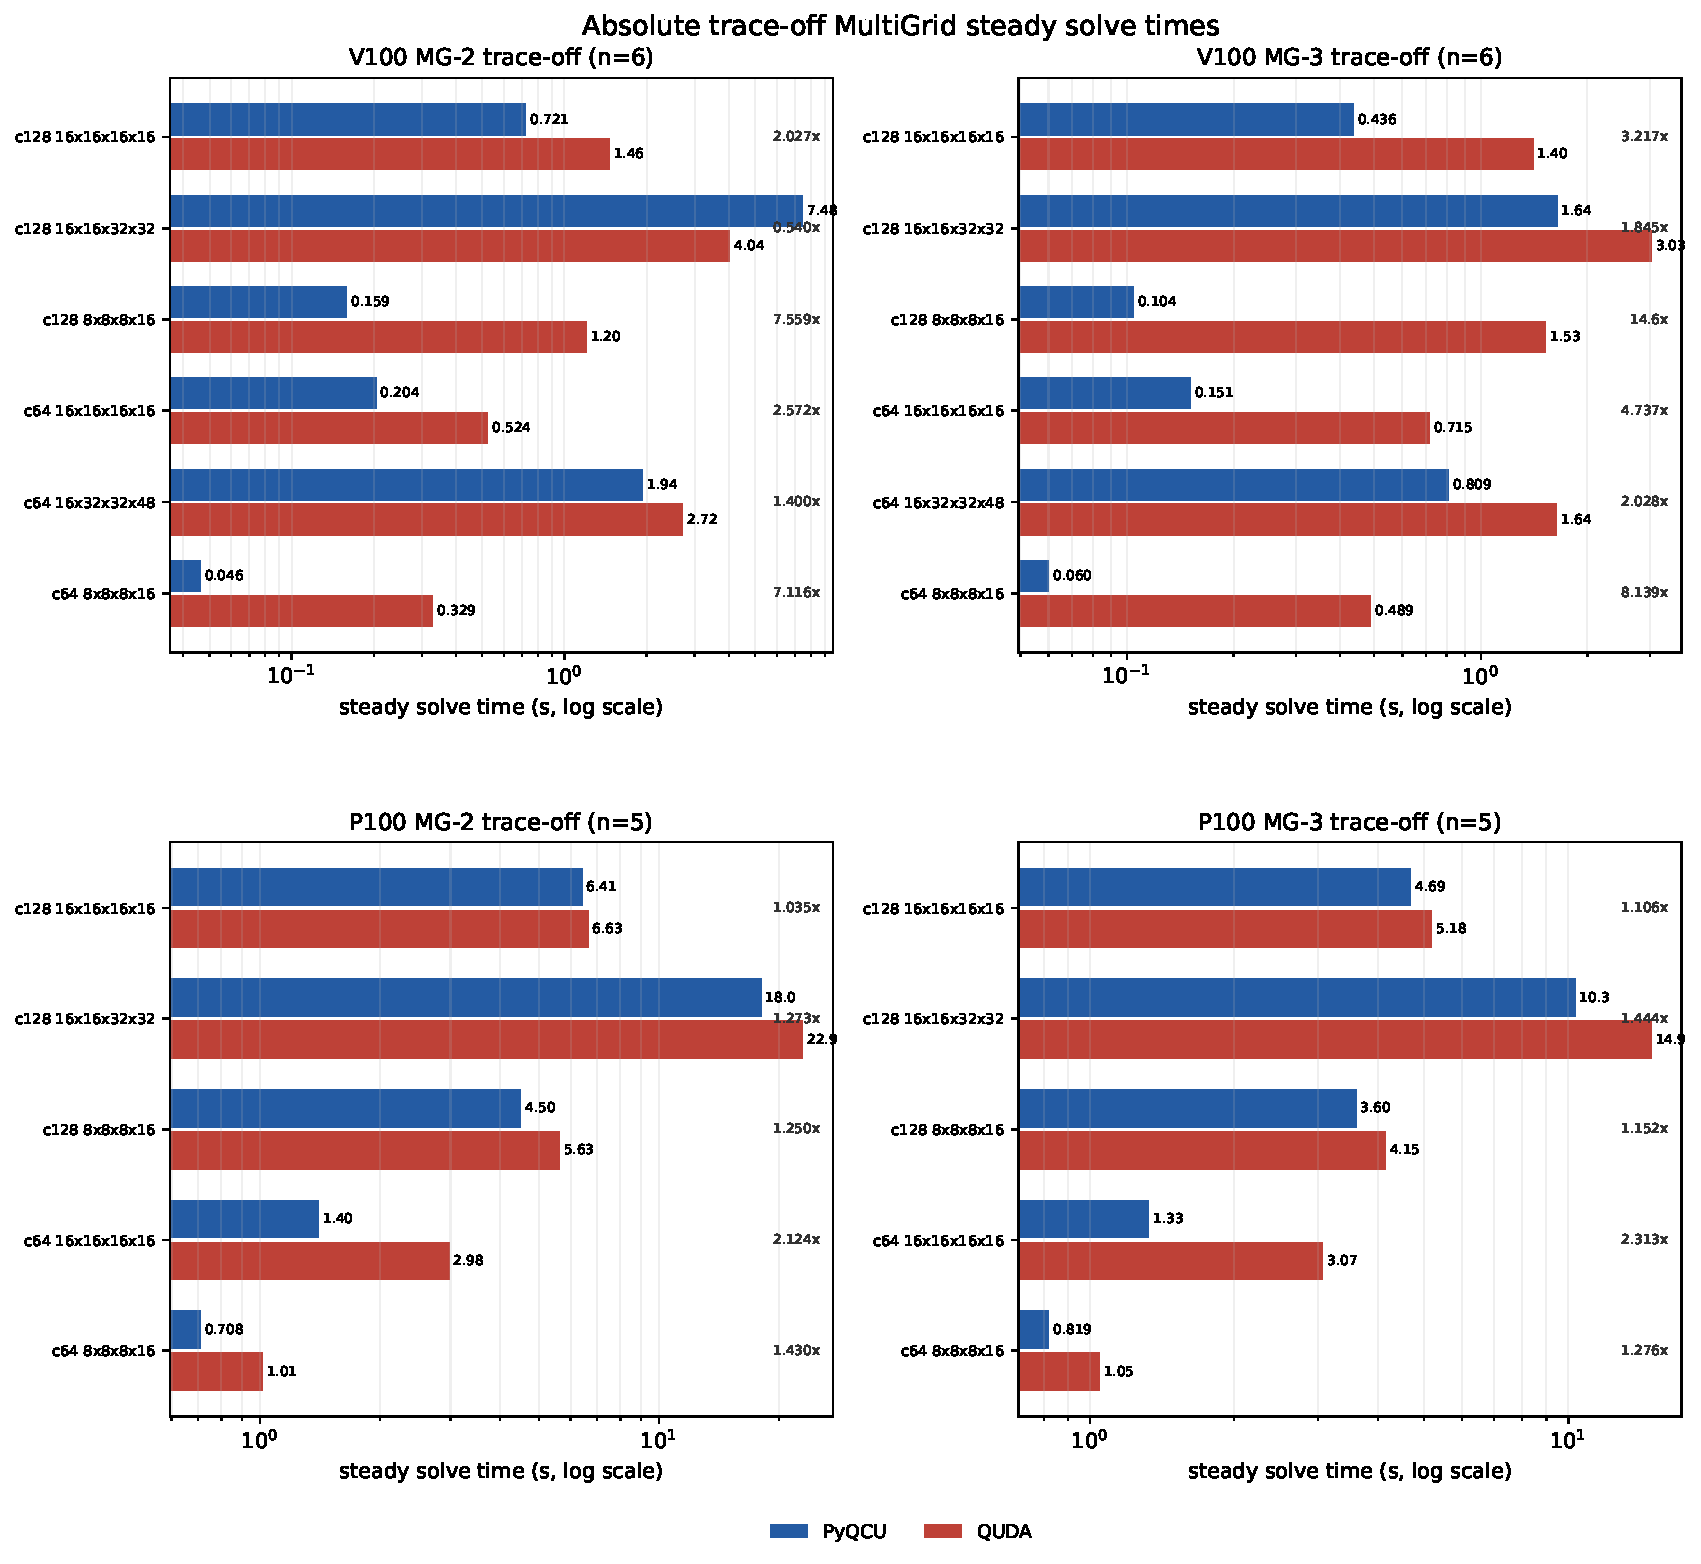
\includegraphics[width=0.98\linewidth,height=0.84\textheight,keepaspectratio]{mg_runtime_traceoff.pdf}
\caption{trace-off MultiGrid 的绝对 steady 耗时重排。四个面板分别对应
V100/P100 与 MG-2/MG-3；每组同排给出 PyQCU 和 QUDA 秒数，右侧给出
$R$。该图替代原宽表式逐单元横轴排列，避免 66 个标签挤在同一坐标轴。}
\label{fig:runtime-traceoff}
\end{figure}

所有精确单元的全局中位时间比为 1.0250。MG-2 为 19/22 个单元优于
QUDA，MG-3 为 16/22，MG-2/3 合计 35/44；BiCGStab 参考为 0/22。
因此 MultiGrid 的组内优势不能外推为 PyQCU 全部求解器优势。

\section{逐层绝对耗时}

逐层数据保留六类原始阶段：pre-smoother、post-smoother、restriction、
prolongation、coarse solver 和 other。图中的 level total 是嵌套记录，
不得跨层直接相加。QUDA 的 trace 会把 2-level 的最粗层 solve 计入
唯一有效层的 coarse 项，并在 3-level 的最后有效层保留最粗层 solve；
本版删除全零占位层，并在图标签中显式写出 \code{/coarsest}，避免原图
把 QUDA 最粗层误读为零。

\begin{figure}[p]
\centering
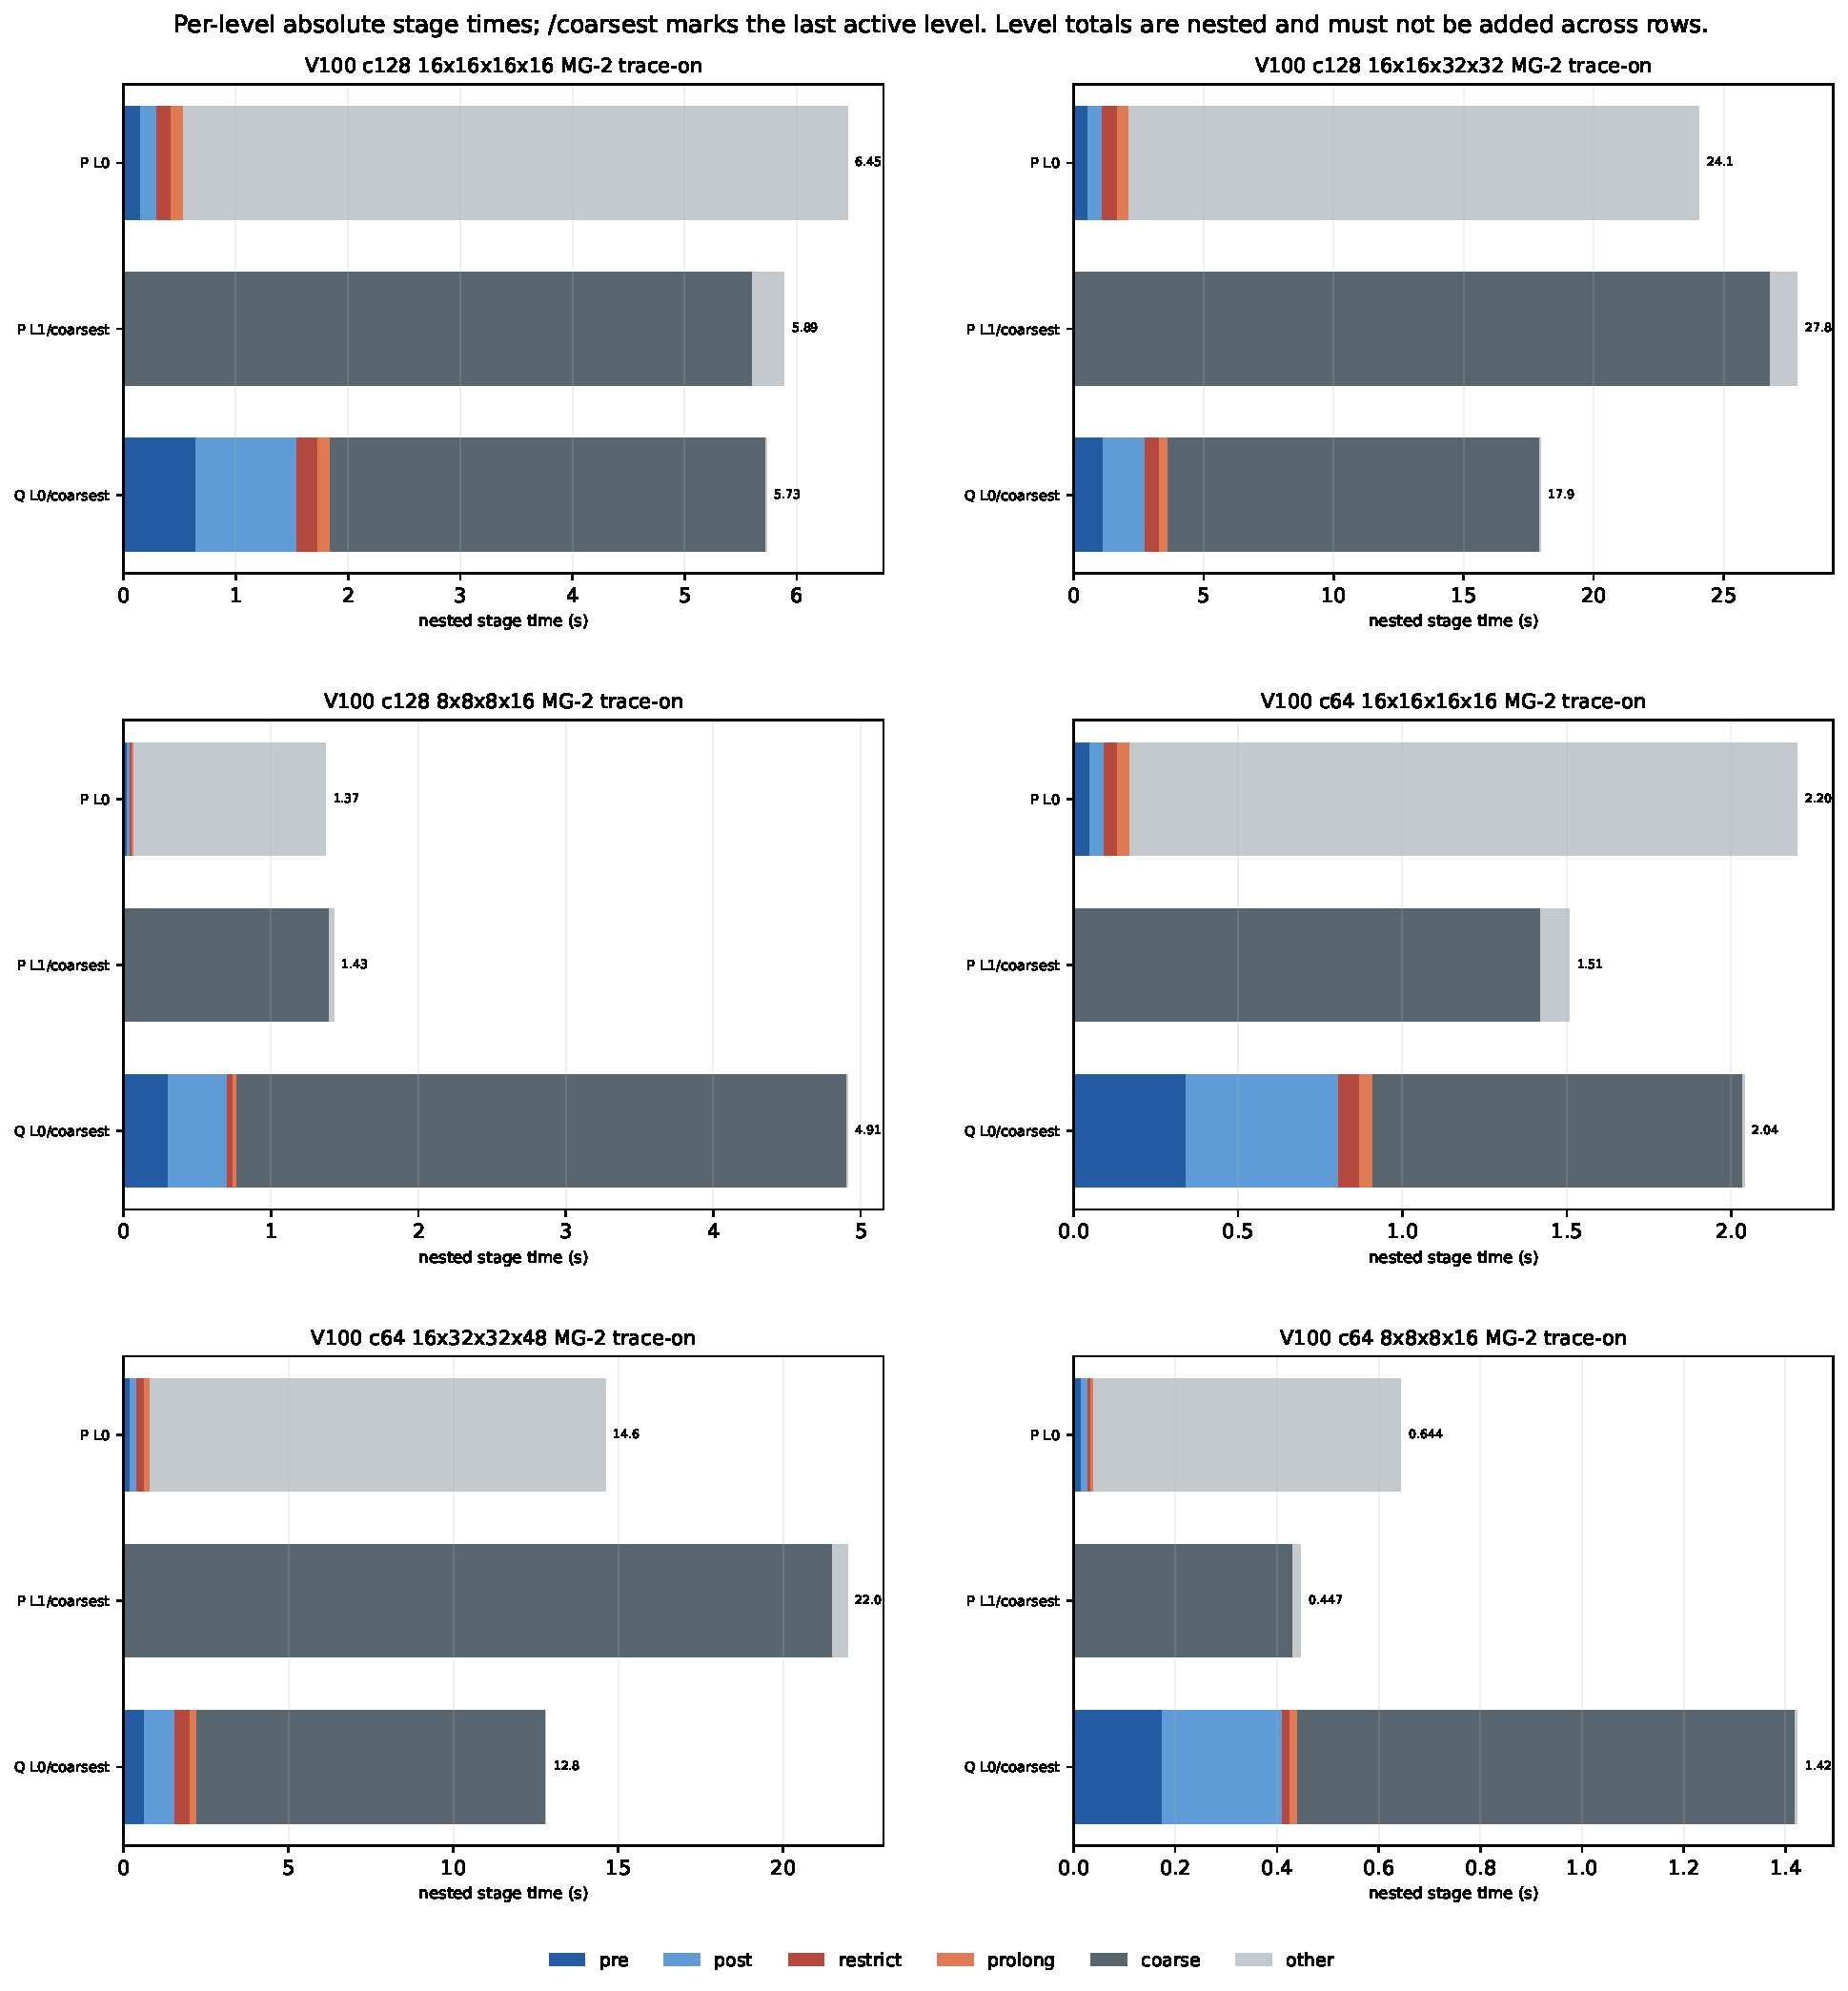
\includegraphics[width=0.98\linewidth,height=0.84\textheight,keepaspectratio]{mg_stage_v100_mg2.pdf}
\caption{逐层绝对阶段耗时：V100 MG-2。P/Q 分别表示 PyQCU/QUDA，
\code{/coarsest} 表示该侧最后一个有效层；颜色给出六类原始阶段。}
\label{fig:stage-times}
\end{figure}

\begin{figure}[p]
\ContinuedFloat
\centering
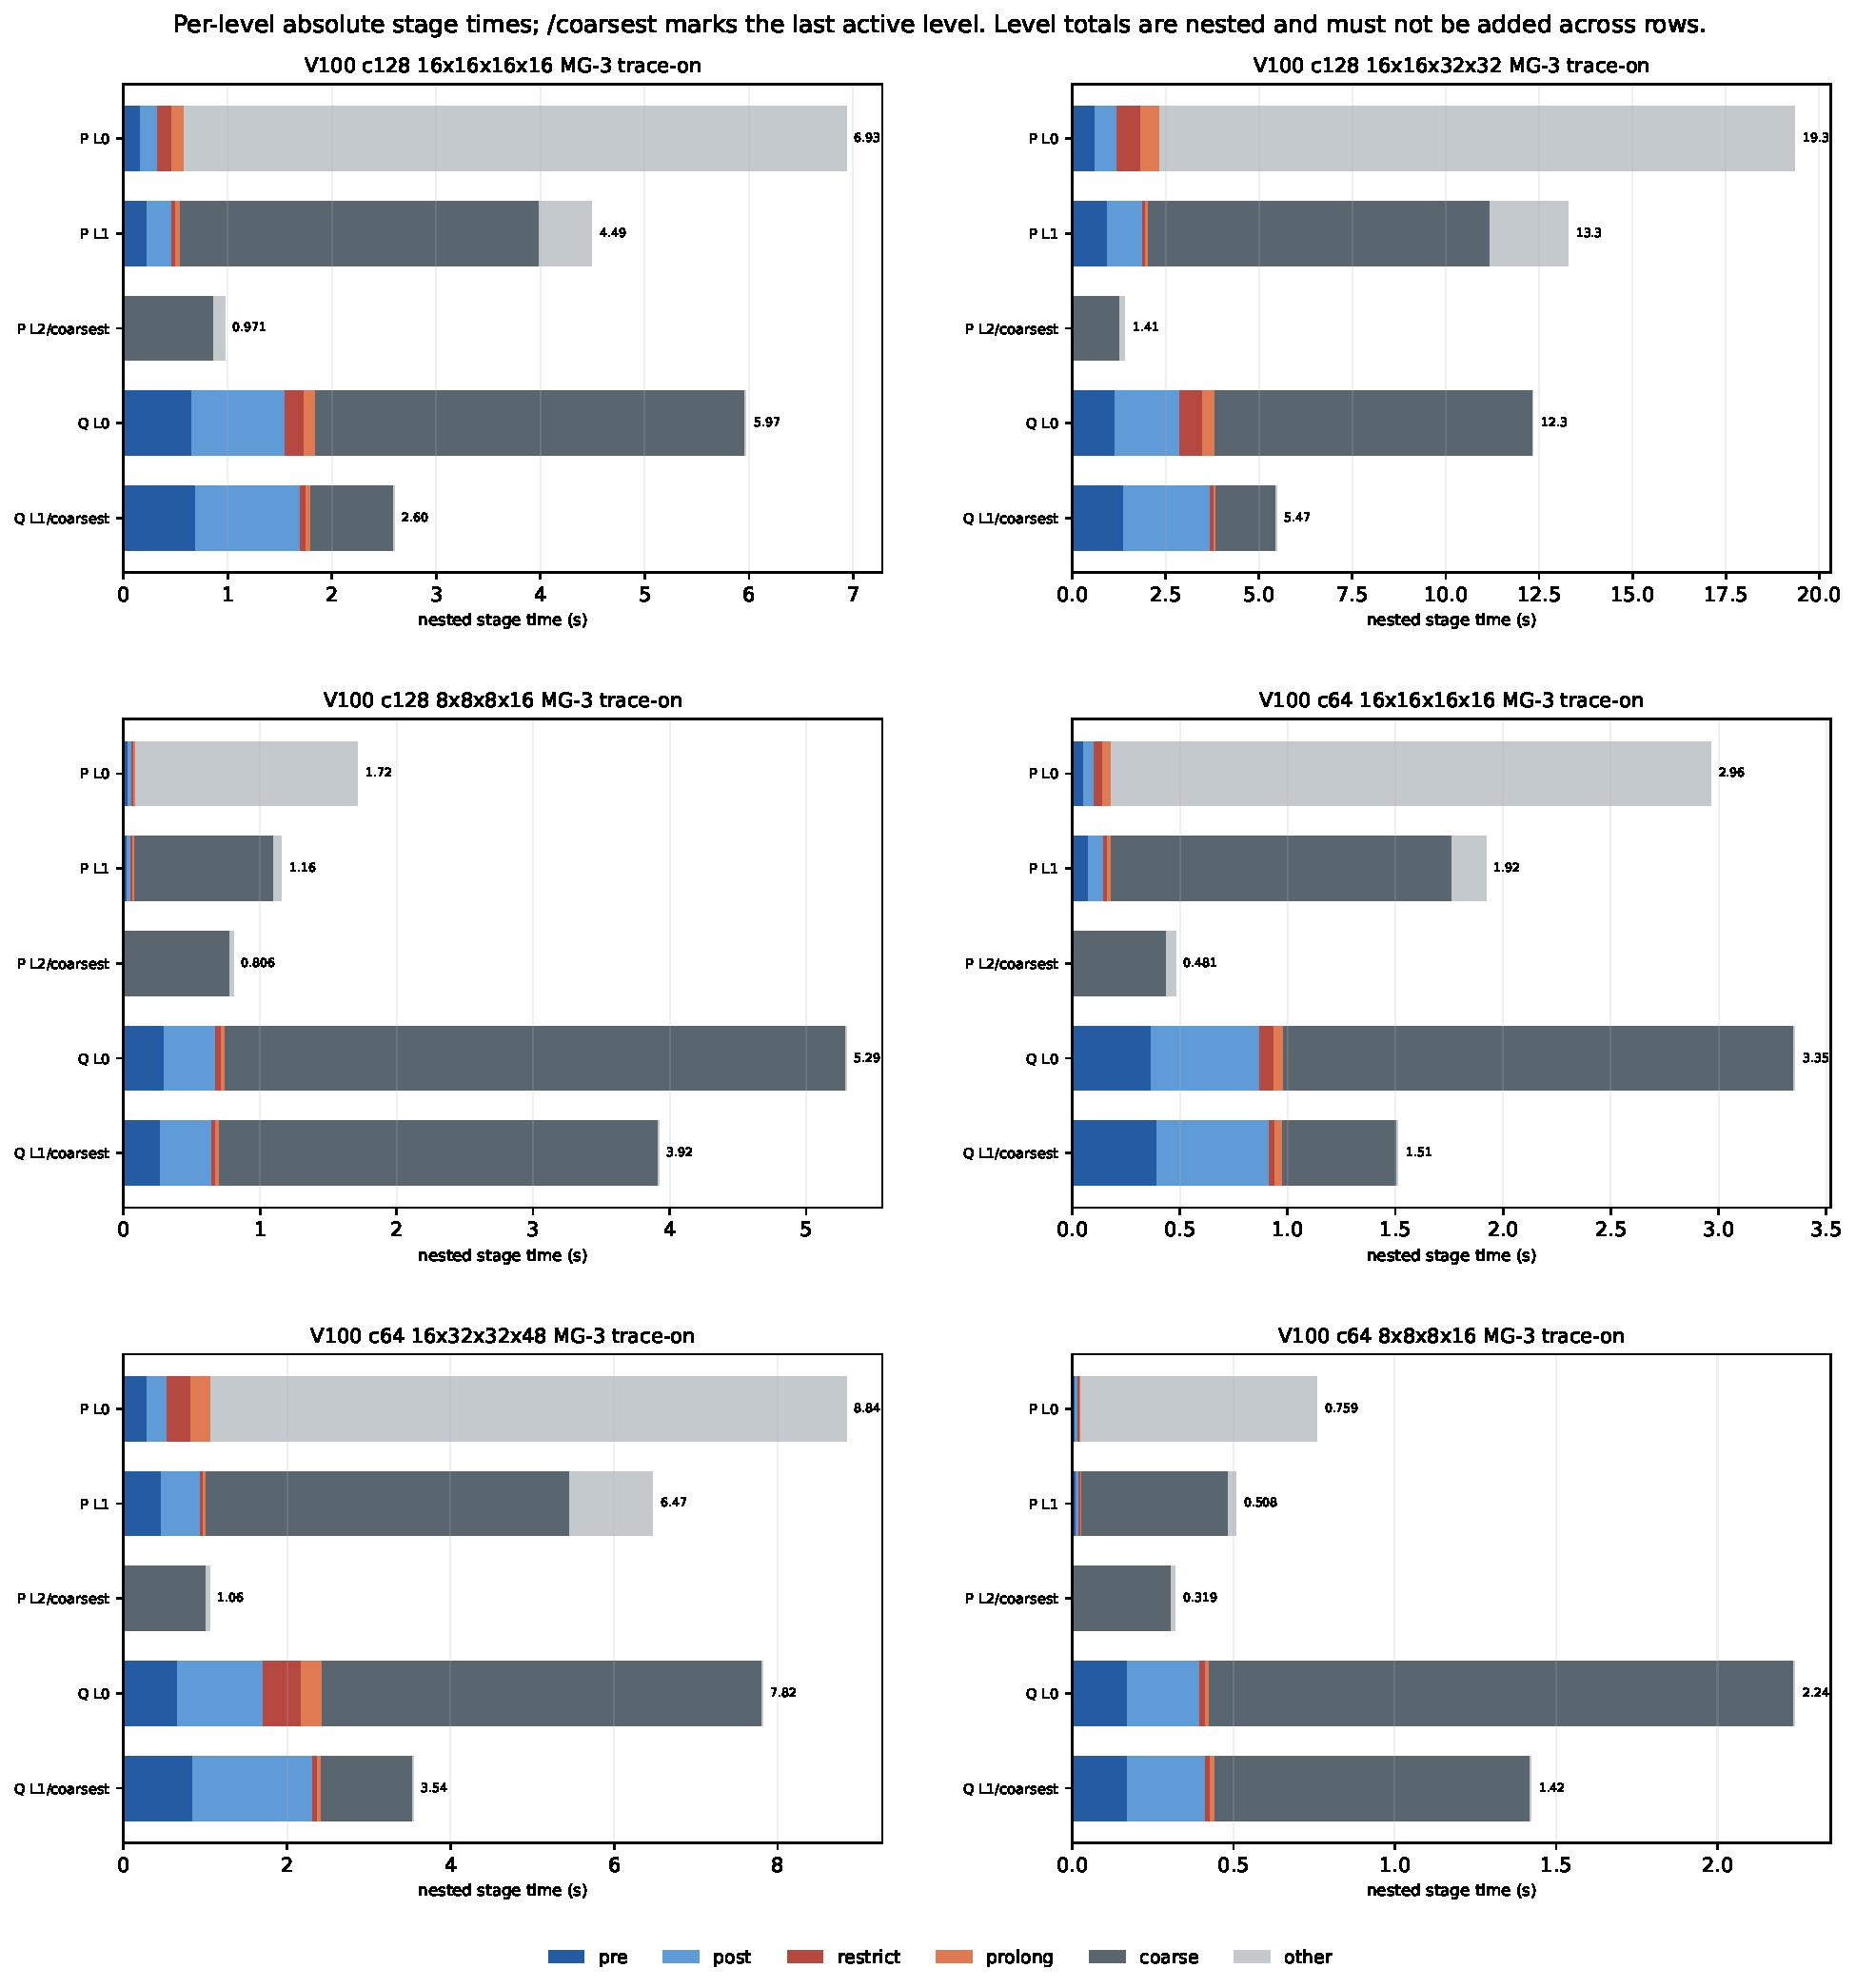
\includegraphics[width=0.98\linewidth,height=0.84\textheight,keepaspectratio]{mg_stage_v100_mg3.pdf}
\caption{（续）V100 MG-3 逐层绝对阶段耗时。}
\end{figure}

\begin{figure}[p]
\ContinuedFloat
\centering
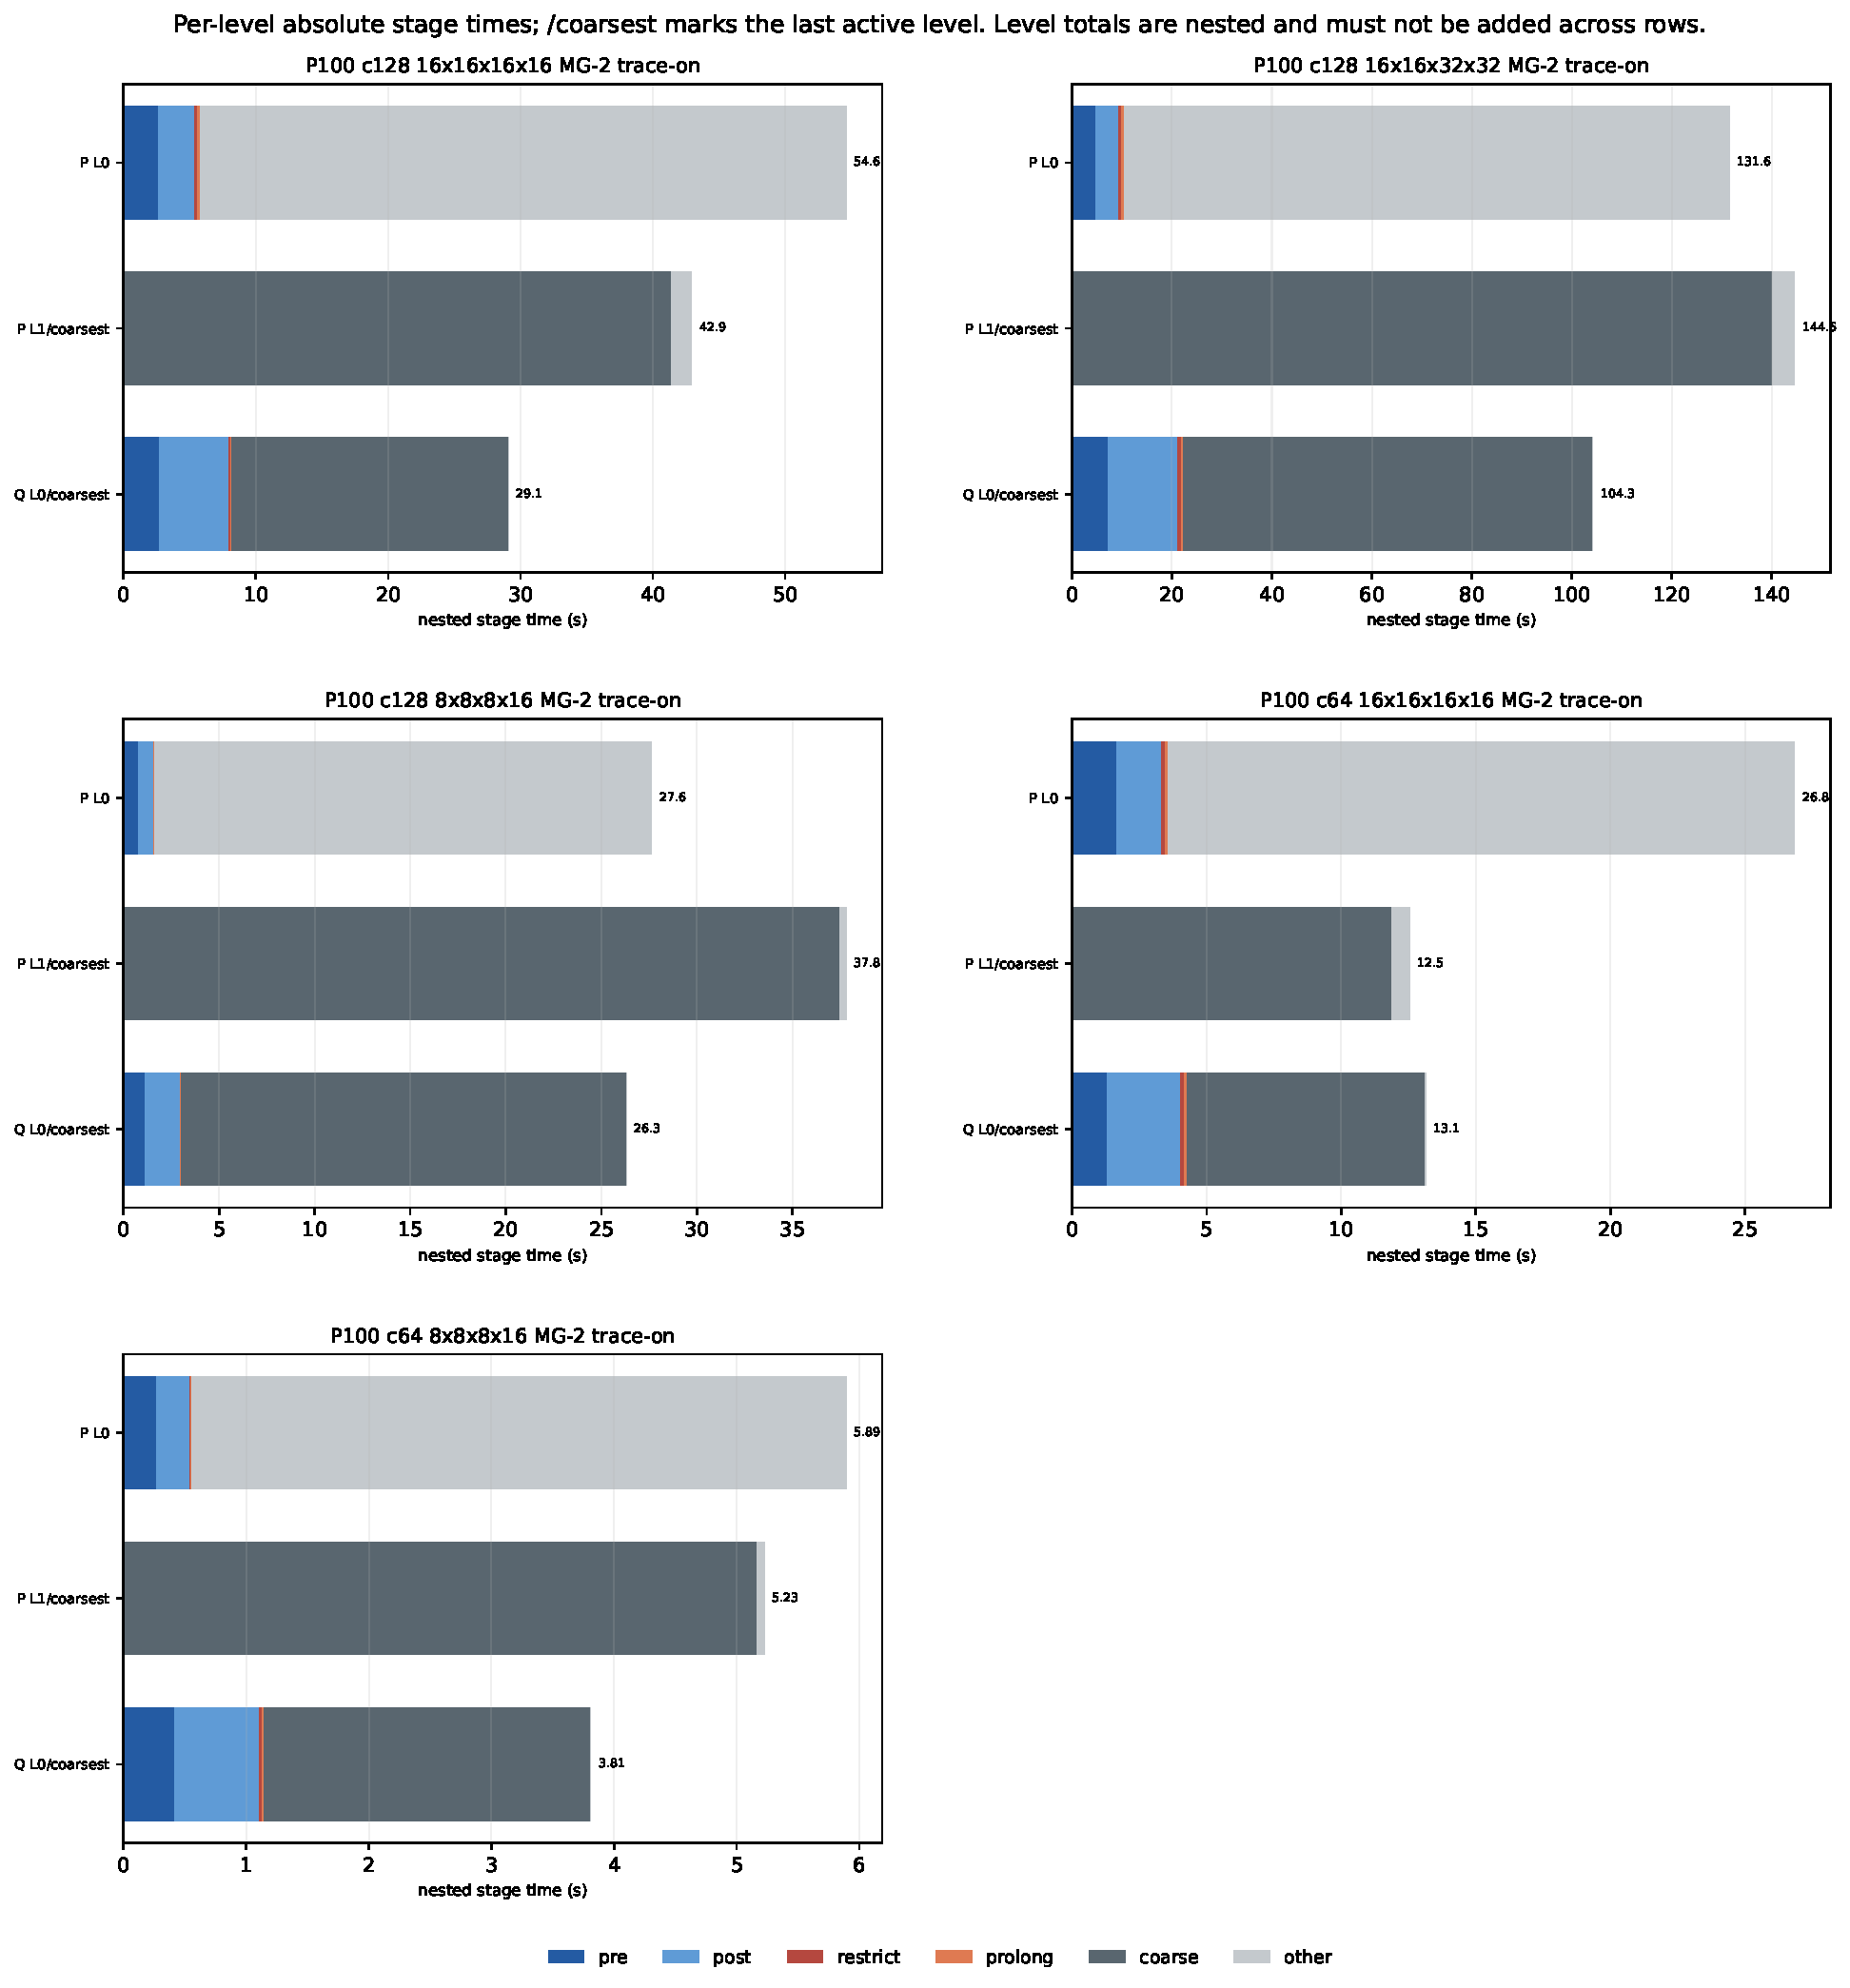
\includegraphics[width=0.98\linewidth,height=0.84\textheight,keepaspectratio]{mg_stage_p100_mg2.pdf}
\caption{（续）P100 MG-2 逐层绝对阶段耗时。}
\end{figure}

\begin{figure}[p]
\ContinuedFloat
\centering
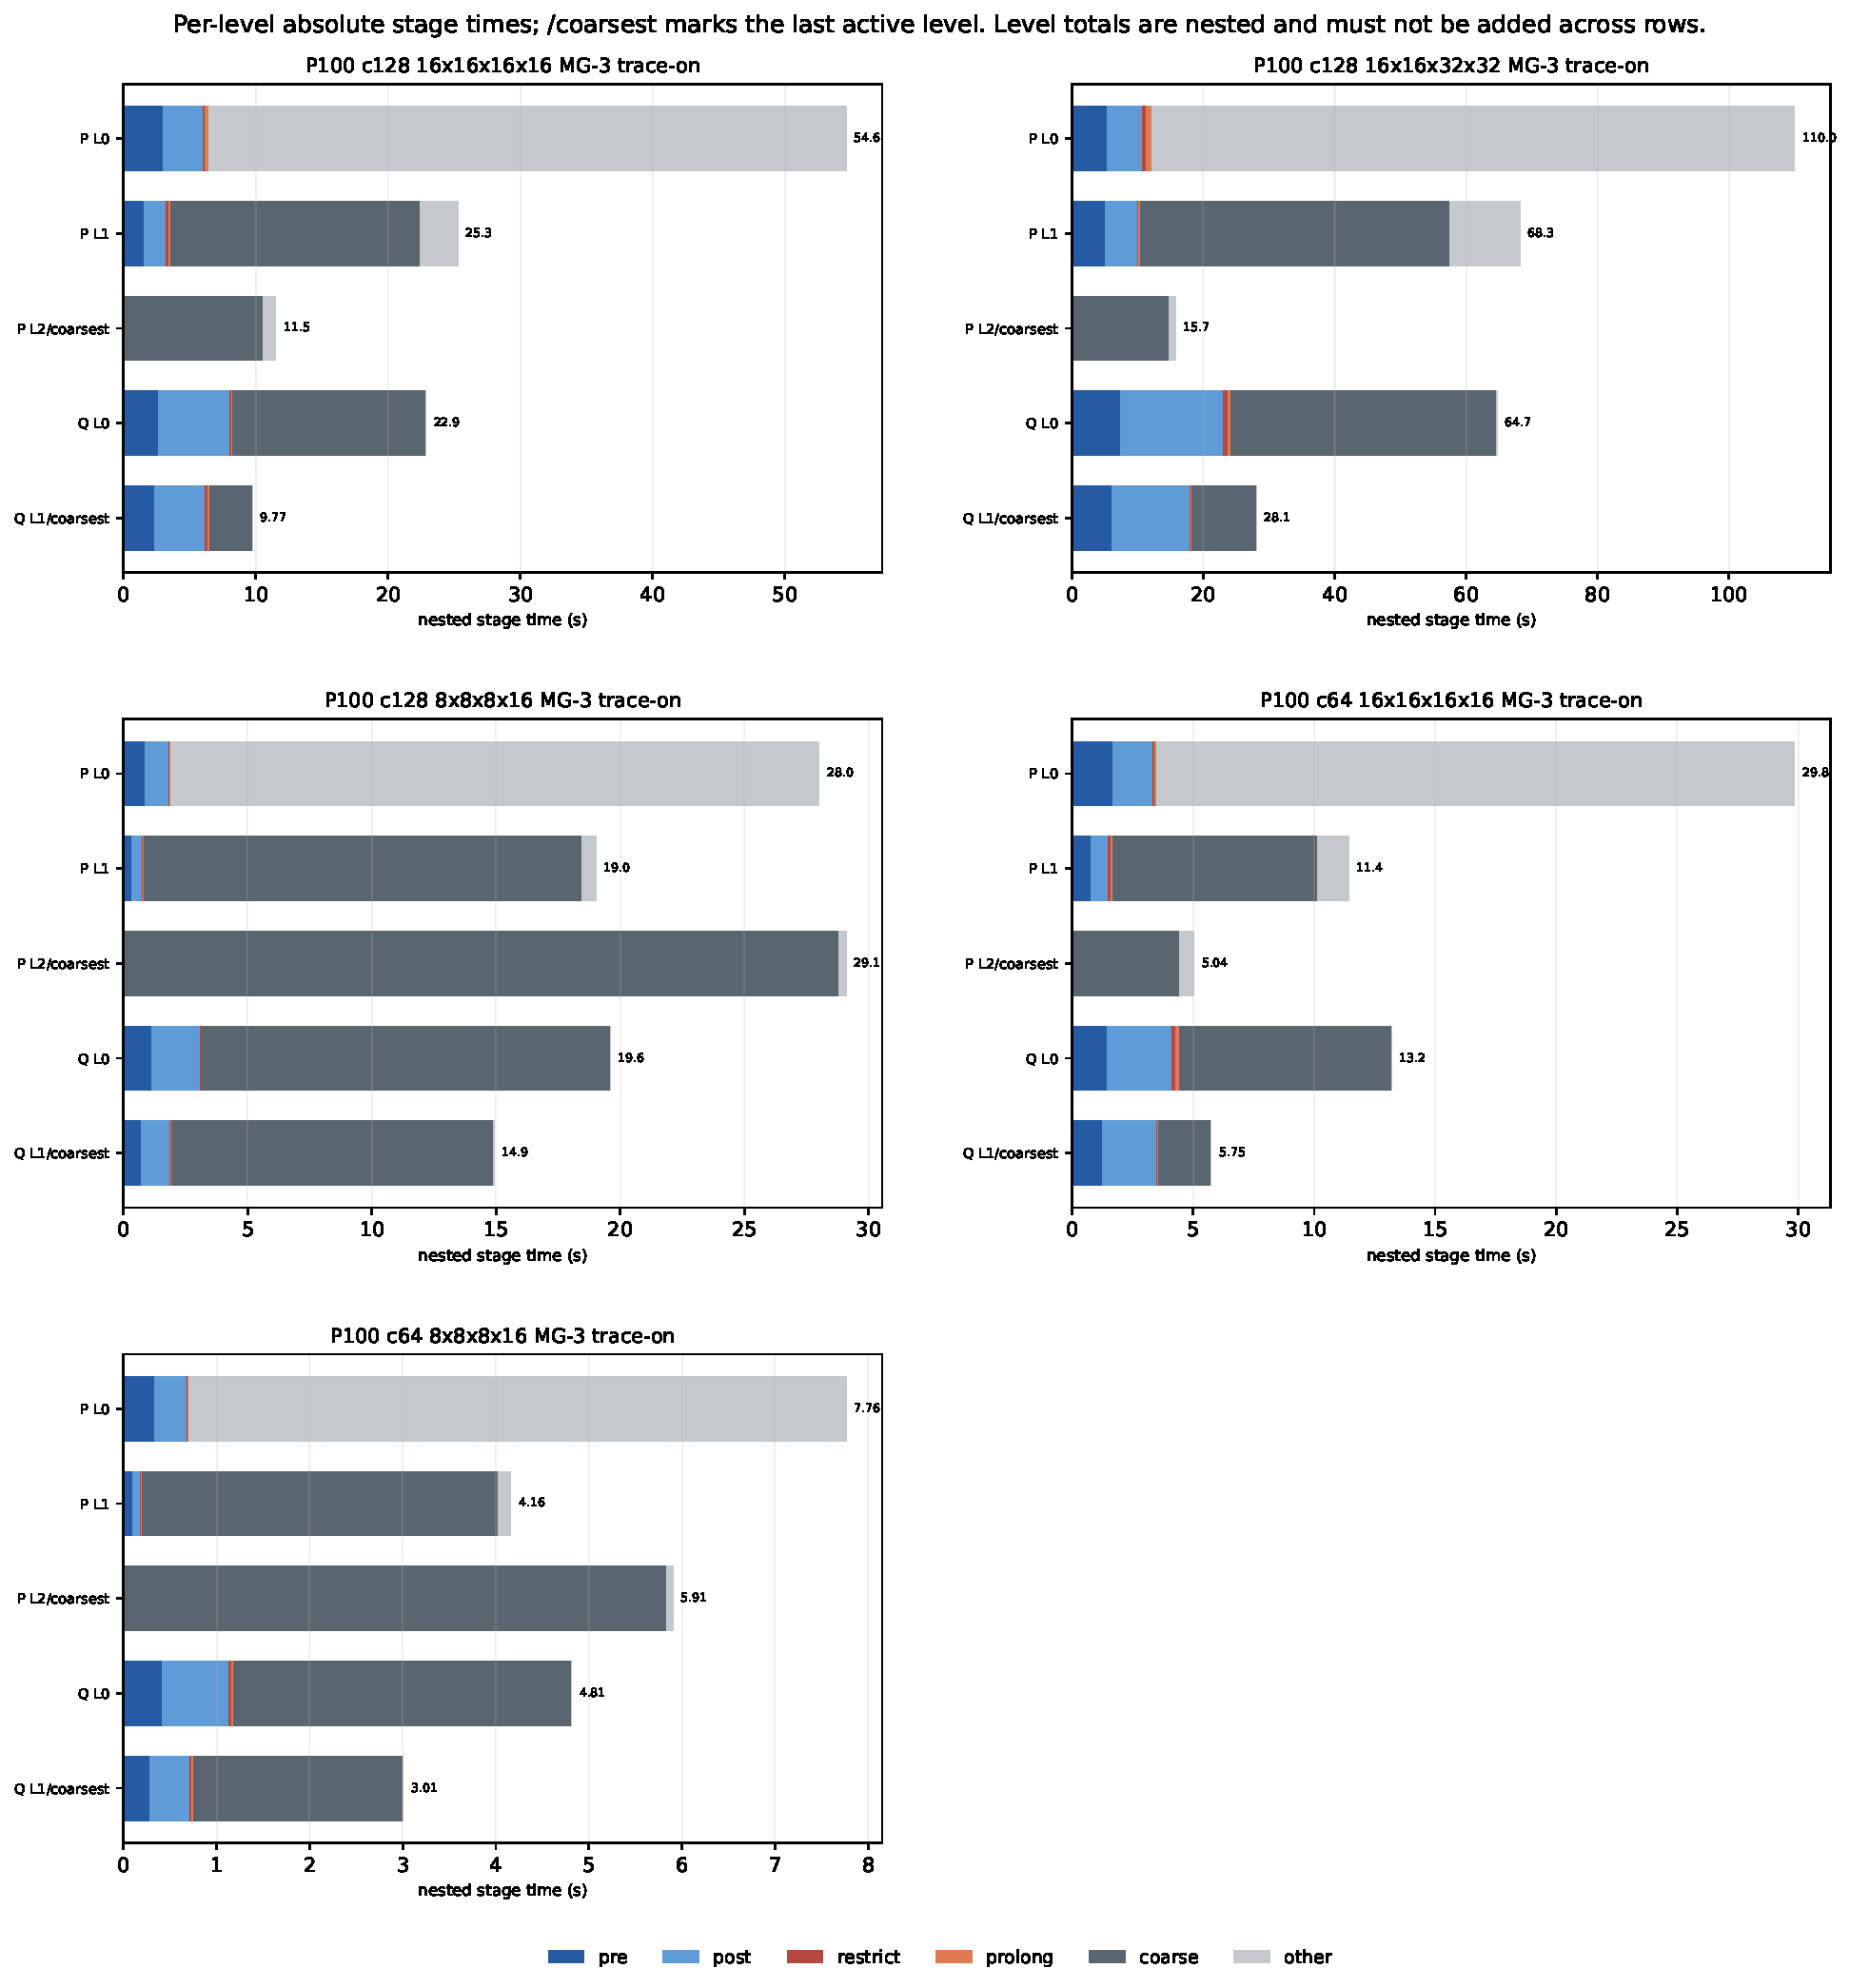
\includegraphics[width=0.98\linewidth,height=0.84\textheight,keepaspectratio]{mg_stage_p100_mg3.pdf}
\caption{（续）P100 MG-3 逐层绝对阶段耗时。}
\end{figure}

\begin{table}[htbp]
\centering
\caption{最粗层 solve 的绝对中位耗时；QUDA 的最后有效层已显式取回}\label{tab:coarsest-times}
\small
\begin{tabular}{@{}llrrrr@{}}
\toprule
设备 & 精度/层数 & $n$ & PyQCU s & QUDA s & $R=Q/P$ \\
\midrule
P100 & c128 / MG-2 & 3 & 41.416 & 23.296 & 0.5625 \\
P100 & c128 / MG-3 & 3 & 14.781 & 9.799 & 0.6629 \\
P100 & c64 / MG-2 & 2 & 8.519 & 5.758 & 0.6758 \\
P100 & c64 / MG-3 & 2 & 5.148 & 2.201 & 0.4275 \\
V100 & c128 / MG-2 & 3 & 5.603 & 4.137 & 0.7384 \\
V100 & c128 / MG-3 & 3 & 0.867 & 1.607 & 1.8538 \\
V100 & c64 / MG-2 & 3 & 1.420 & 1.124 & 0.7917 \\
V100 & c64 / MG-3 & 3 & 0.438 & 0.977 & 2.2279 \\
\bottomrule
\end{tabular}
\end{table}


最粗层表中 PyQCU 与 QUDA 都取各自最后有效层的
\code{coarse_solver_seconds}。例如 P100 c128 MG-3 的 PyQCU 与 QUDA
中位最粗层 solve 分别为 14.781 s 和 9.799 s，说明该组合的粗层是
PyQCU 的明确薄弱项；相对地，V100 c64 MG-3 分别为 0.438 s 和
0.977 s，此时 PyQCU 在粗层反占优。

完整的逐 side、逐 level 六项耗时保留在
\path{stage_times.csv}。下表给出按设备、精度、MG 层数、侧和 level
聚合的中位值；\code{Total} 是六项在同一条嵌套记录内的和。

\begin{landscape}
\begin{longtable}{@{}lllrrrrrrrrrr@{}}
\caption{MG level component medians (seconds; trace-on, nested)}\label{tab:stage-components}\\
\toprule
Device & Prec & MG & Side & L & $n$ & Pre & Post & Restrict & Prolong & Coarse & Other & Total \\
\midrule
\endfirsthead
\toprule
Device & Prec & MG & Side & L & $n$ & Pre & Post & Restrict & Prolong & Coarse & Other & Total \\
\midrule
\endhead
P100 & c128 & MG-2 & PyQCU & L0 & 3 & 2.649 & 2.725 & 0.208 & 0.227 & 0.000 & 48.804 & 54.612 \\
P100 & c128 & MG-2 & PyQCU & L1 & 3 & 0.000 & 0.000 & 0.000 & 0.000 & 41.416 & 1.515 & 42.931 \\
P100 & c128 & MG-2 & QUDA & L0 & 3 & 2.714 & 5.226 & 0.135 & 0.098 & 23.296 & 0.011 & 31.478 \\
P100 & c128 & MG-3 & PyQCU & L0 & 3 & 3.013 & 2.989 & 0.182 & 0.244 & 0.000 & 48.206 & 54.634 \\
P100 & c128 & MG-3 & PyQCU & L1 & 3 & 1.592 & 1.650 & 0.102 & 0.088 & 18.855 & 2.897 & 25.185 \\
P100 & c128 & MG-3 & PyQCU & L2 & 3 & 0.000 & 0.000 & 0.000 & 0.000 & 14.781 & 0.927 & 15.708 \\
P100 & c128 & MG-3 & QUDA & L0 & 3 & 2.654 & 5.405 & 0.106 & 0.082 & 16.455 & 0.011 & 24.713 \\
P100 & c128 & MG-3 & QUDA & L1 & 3 & 2.382 & 3.805 & 0.131 & 0.100 & 9.799 & 0.011 & 16.227 \\
P100 & c64 & MG-2 & PyQCU & L0 & 2 & 0.964 & 0.969 & 0.066 & 0.057 & 0.000 & 14.313 & 16.369 \\
P100 & c64 & MG-2 & PyQCU & L1 & 2 & 0.000 & 0.000 & 0.000 & 0.000 & 8.519 & 0.365 & 8.885 \\
P100 & c64 & MG-2 & QUDA & L0 & 2 & 0.865 & 1.706 & 0.089 & 0.053 & 5.758 & 0.005 & 8.475 \\
P100 & c64 & MG-3 & PyQCU & L0 & 2 & 1.018 & 0.986 & 0.048 & 0.054 & 0.000 & 16.701 & 18.807 \\
P100 & c64 & MG-3 & PyQCU & L1 & 2 & 0.440 & 0.396 & 0.061 & 0.045 & 6.134 & 0.722 & 7.799 \\
P100 & c64 & MG-3 & PyQCU & L2 & 2 & 0.000 & 0.000 & 0.000 & 0.000 & 5.148 & 0.325 & 5.472 \\
P100 & c64 & MG-3 & QUDA & L0 & 2 & 0.932 & 1.698 & 0.087 & 0.104 & 6.180 & 0.005 & 9.006 \\
P100 & c64 & MG-3 & QUDA & L1 & 2 & 0.781 & 1.333 & 0.032 & 0.027 & 2.201 & 0.005 & 4.378 \\
V100 & c128 & MG-2 & PyQCU & L0 & 3 & 0.147 & 0.150 & 0.124 & 0.113 & 0.000 & 5.917 & 6.452 \\
V100 & c128 & MG-2 & PyQCU & L1 & 3 & 0.000 & 0.000 & 0.000 & 0.000 & 5.603 & 0.284 & 5.887 \\
V100 & c128 & MG-2 & QUDA & L0 & 3 & 0.645 & 0.901 & 0.182 & 0.116 & 4.137 & 0.010 & 5.991 \\
V100 & c128 & MG-3 & PyQCU & L0 & 3 & 0.166 & 0.158 & 0.143 & 0.112 & 0.000 & 6.355 & 6.934 \\
V100 & c128 & MG-3 & PyQCU & L1 & 3 & 0.228 & 0.234 & 0.043 & 0.043 & 3.439 & 0.509 & 4.494 \\
V100 & c128 & MG-3 & PyQCU & L2 & 3 & 0.000 & 0.000 & 0.000 & 0.000 & 0.867 & 0.104 & 0.971 \\
V100 & c128 & MG-3 & QUDA & L0 & 3 & 0.652 & 0.895 & 0.182 & 0.114 & 4.544 & 0.010 & 6.396 \\
V100 & c128 & MG-3 & QUDA & L1 & 3 & 0.692 & 0.999 & 0.058 & 0.051 & 1.607 & 0.010 & 3.418 \\
V100 & c64 & MG-2 & PyQCU & L0 & 3 & 0.049 & 0.045 & 0.039 & 0.039 & 0.000 & 2.029 & 2.201 \\
V100 & c64 & MG-2 & PyQCU & L1 & 3 & 0.000 & 0.000 & 0.000 & 0.000 & 1.420 & 0.088 & 1.508 \\
V100 & c64 & MG-2 & QUDA & L0 & 3 & 0.342 & 0.463 & 0.064 & 0.040 & 1.124 & 0.005 & 2.039 \\
V100 & c64 & MG-3 & PyQCU & L0 & 3 & 0.054 & 0.047 & 0.041 & 0.040 & 0.000 & 2.782 & 2.965 \\
V100 & c64 & MG-3 & PyQCU & L1 & 3 & 0.076 & 0.071 & 0.018 & 0.014 & 1.582 & 0.159 & 1.921 \\
V100 & c64 & MG-3 & PyQCU & L2 & 3 & 0.000 & 0.000 & 0.000 & 0.000 & 0.438 & 0.043 & 0.481 \\
V100 & c64 & MG-3 & QUDA & L0 & 3 & 0.368 & 0.500 & 0.069 & 0.045 & 2.365 & 0.005 & 3.353 \\
V100 & c64 & MG-3 & QUDA & L1 & 3 & 0.394 & 0.518 & 0.030 & 0.034 & 0.977 & 0.006 & 1.959 \\
\bottomrule
\end{longtable}

\end{landscape}

\section{峰值显存}

下表使用每个 side-case 的不计时 device-wide sampler
\code{device_used_max_observed_bytes}。该值可能包含测试进程之外的
同设备分配，因此只用于门限检查，不声明为进程独占峰值。

\begin{table}[htbp]
\centering
\caption{峰值 device-wide 显存（MiB）}
\small
\begin{tabular}{@{}llrrr@{}}
\toprule
侧 & 设备/精度 & 样本 & median & max \\
\midrule
PyQCU & P100/c64 & 12 & 1852.9 & 2134.9 \\
PyQCU & P100/c128 & 18 & 3150.9 & 7308.9 \\
PyQCU & V100/c64 & 18 & 2677.3 & 11907.3 \\
PyQCU & V100/c128 & 18 & 4005.3 & 9575.3 \\
QUDA & P100/c64 & 12 & 1934.9 & 2628.9 \\
QUDA & P100/c128 & 18 & 3800.9 & 11082.9 \\
QUDA & V100/c64 & 18 & 3587.3 & 23063.3 \\
QUDA & V100/c128 & 18 & 5227.3 & 15739.3 \\
\bottomrule
\end{tabular}
\end{table}

\begin{figure}[htbp]
\centering
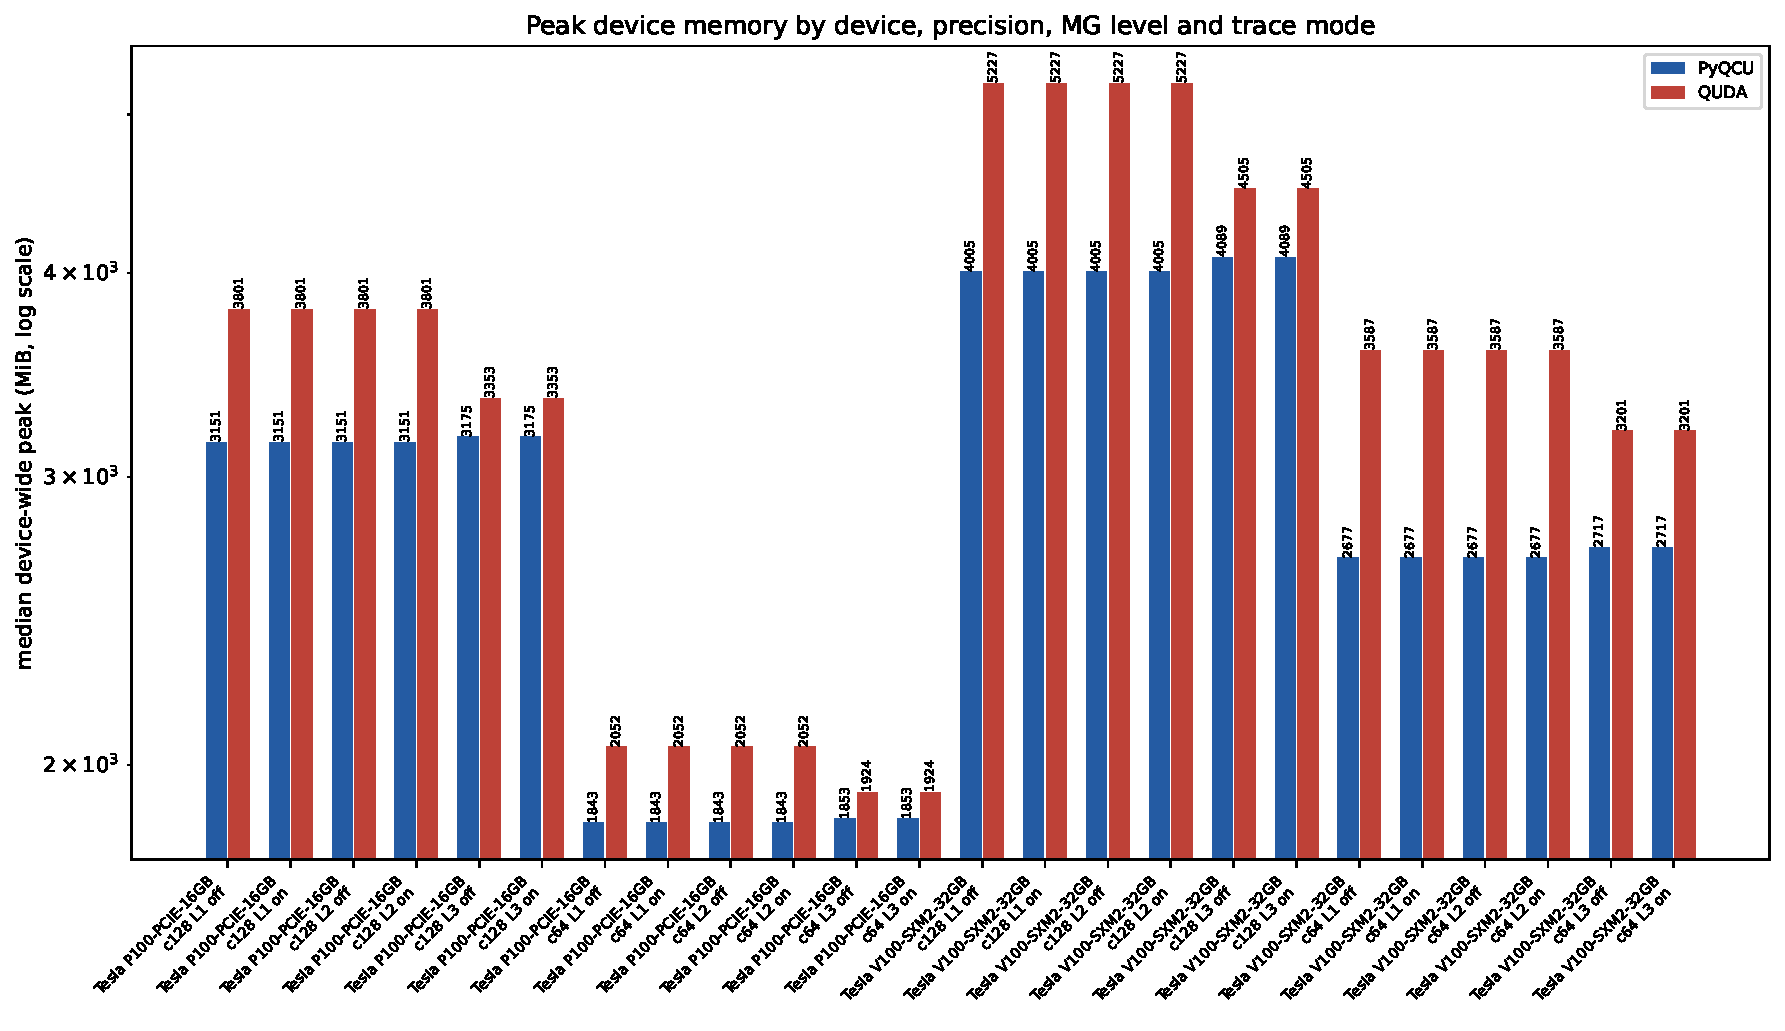
\includegraphics[width=0.98\linewidth,height=0.70\textheight,keepaspectratio]{mg_peak_memory.pdf}
\caption{设备级峰值显存按设备、精度、MG 层数和 trace 模式的中位数。}
\label{fig:peak-memory}
\end{figure}

精确单元中最大的 PyQCU 观测峰值约 11.9 GiB，占 V100 容量 36.3\%；
最大 QUDA 观测峰值约 23.1 GiB，占 V100 容量 70.4\%。保留结果均低于
85\% 门限。逐 side、setup、first solve、steady、allocator 与 workspace
原值见 \path{mg_memory.csv}。

\section{残差收敛}

\begin{table}[htbp]
\centering
\caption{稳态最细层 full true residual}
\small
\begin{tabular}{@{}lrrr@{}}
\toprule
侧 & 样本 & median & max \\
\midrule
PyQCU & 66 & $1.85\times10^{-8}$ & $7.40\times10^{-7}$ \\
QUDA & 66 & $1.89\times10^{-8}$ & $7.97\times10^{-7}$ \\
\bottomrule
\end{tabular}
\end{table}

\begin{figure}[p]
\centering
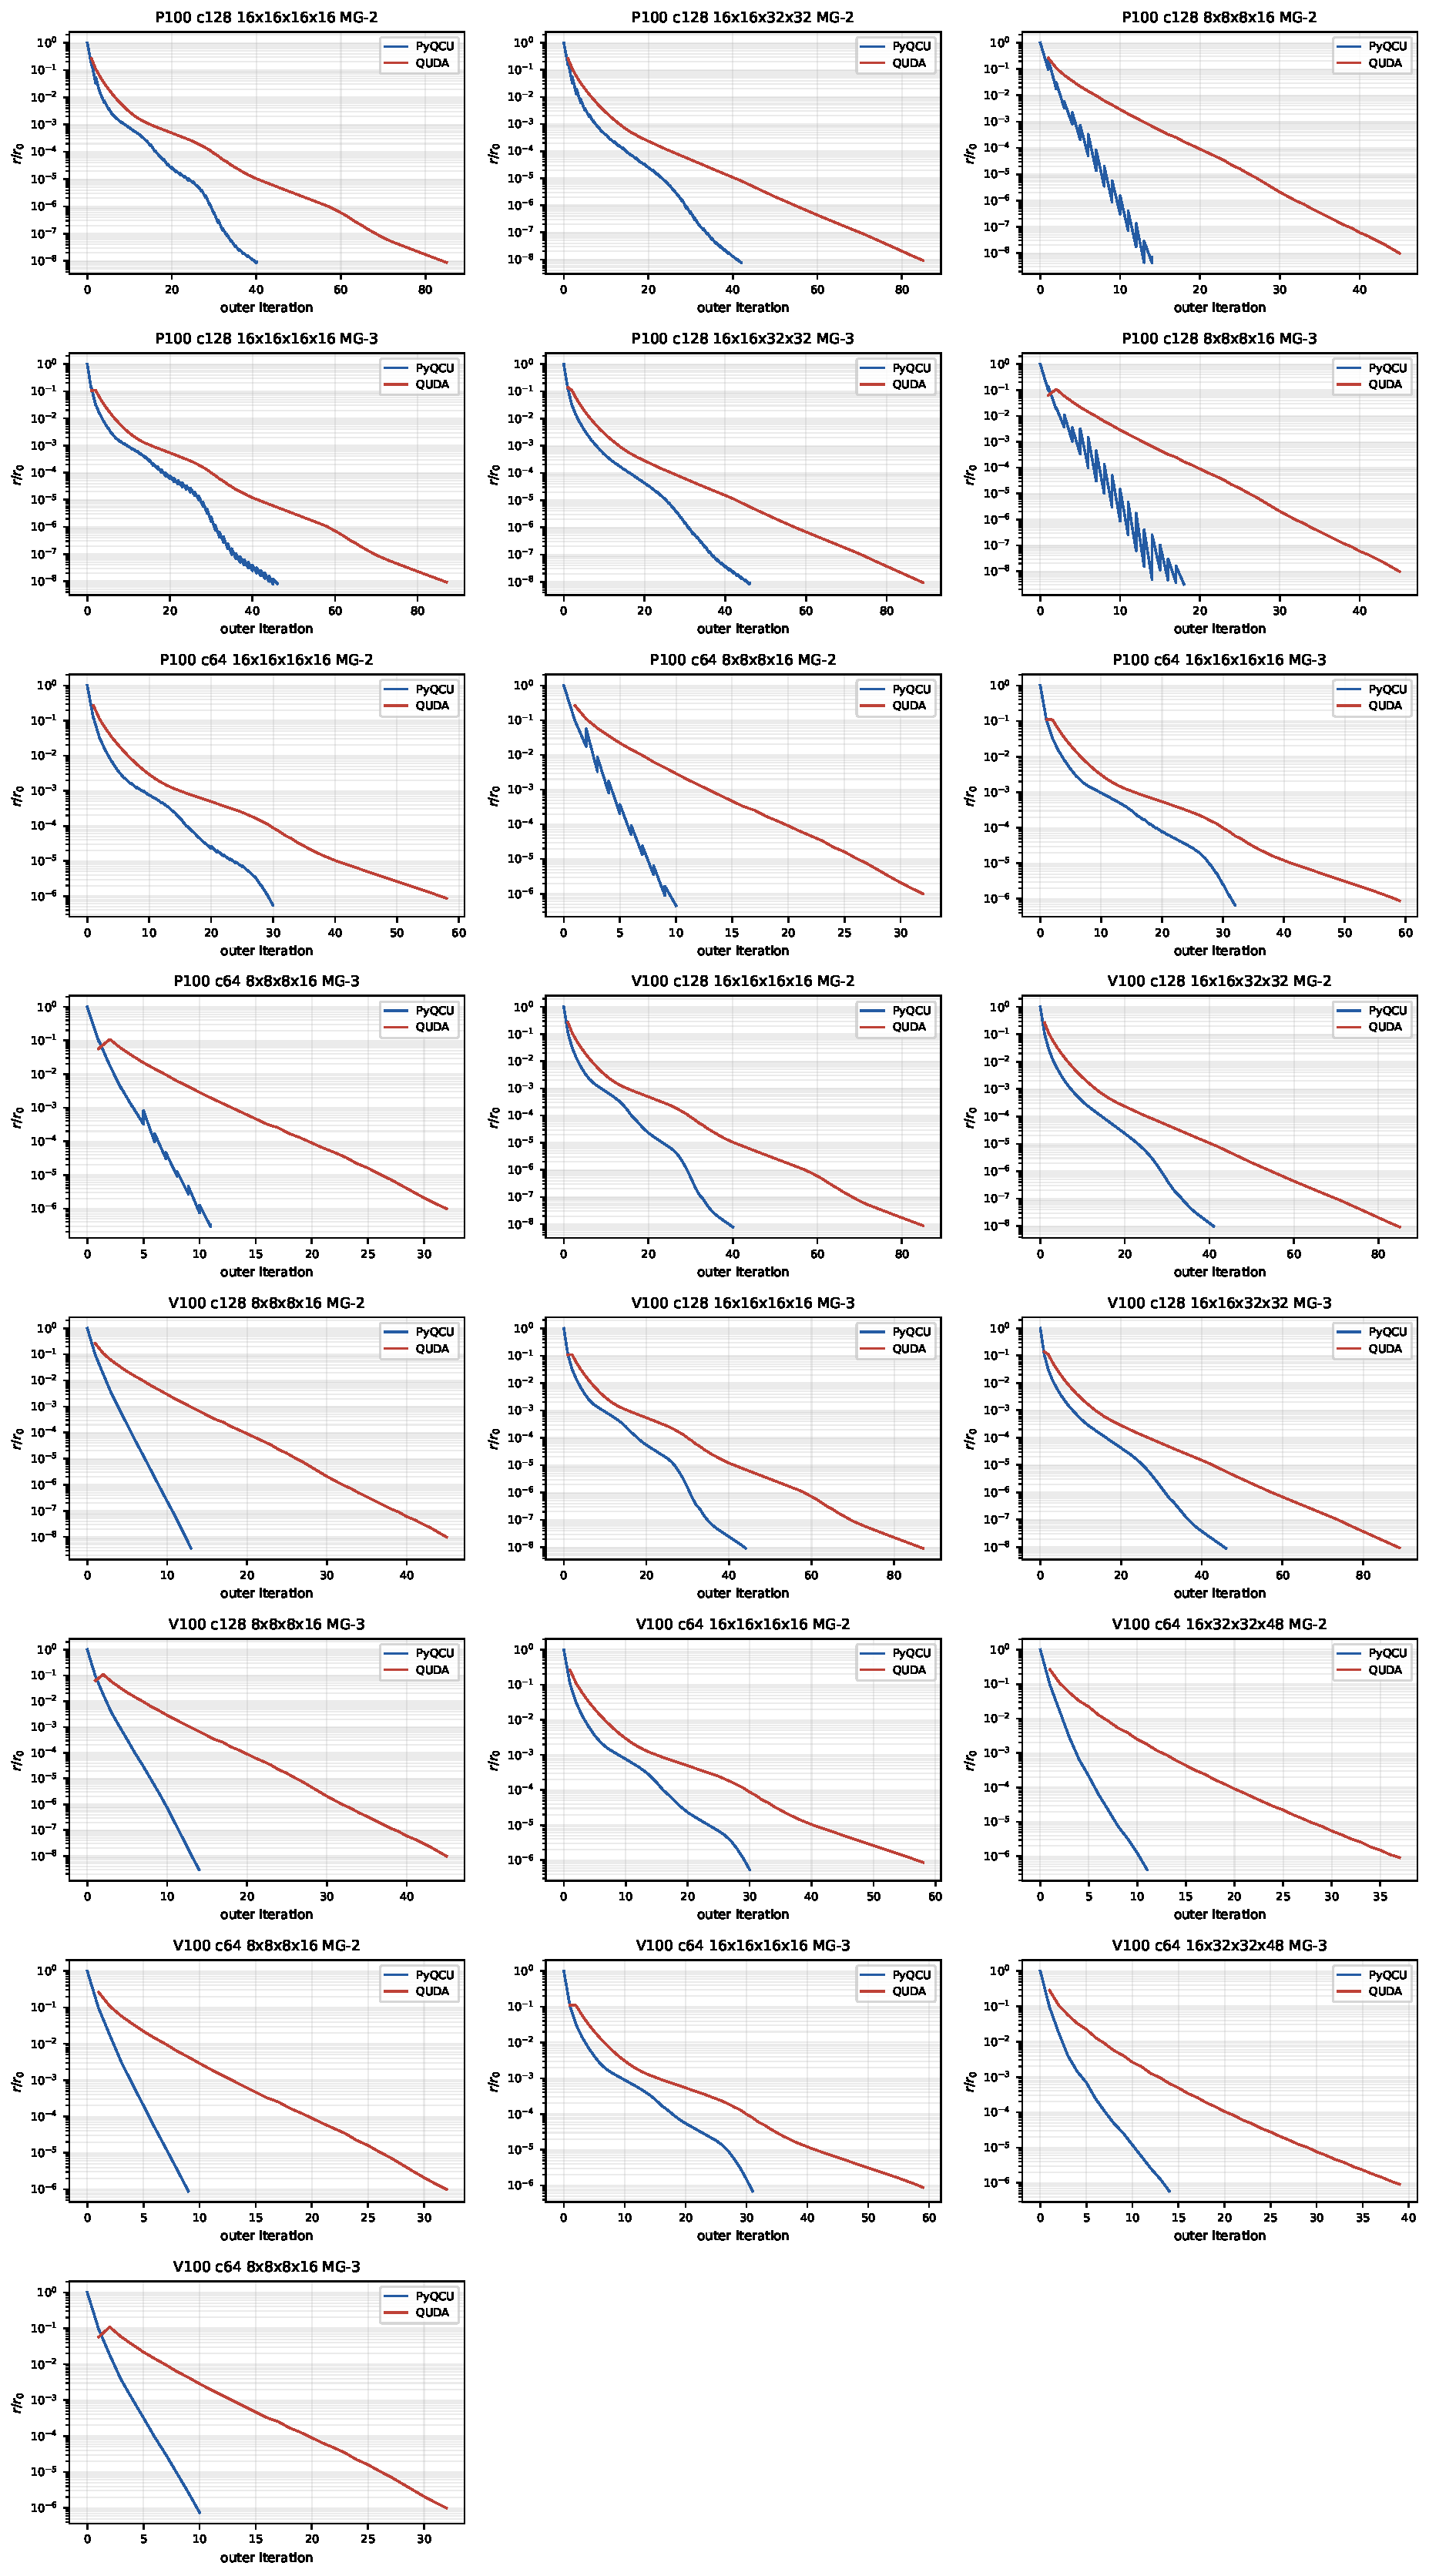
\includegraphics[width=0.96\linewidth,height=0.82\textheight,keepaspectratio]{mg_residual_curves.pdf}
\caption{全部 44 个 trace-on MG-2/3 side 的最细层收敛小面板。
每个面板内只对比 PyQCU 与 QUDA，避免 44 条曲线的图例互相遮挡。}
\label{fig:residual-panels}
\end{figure}

\begin{figure}[p]
\centering
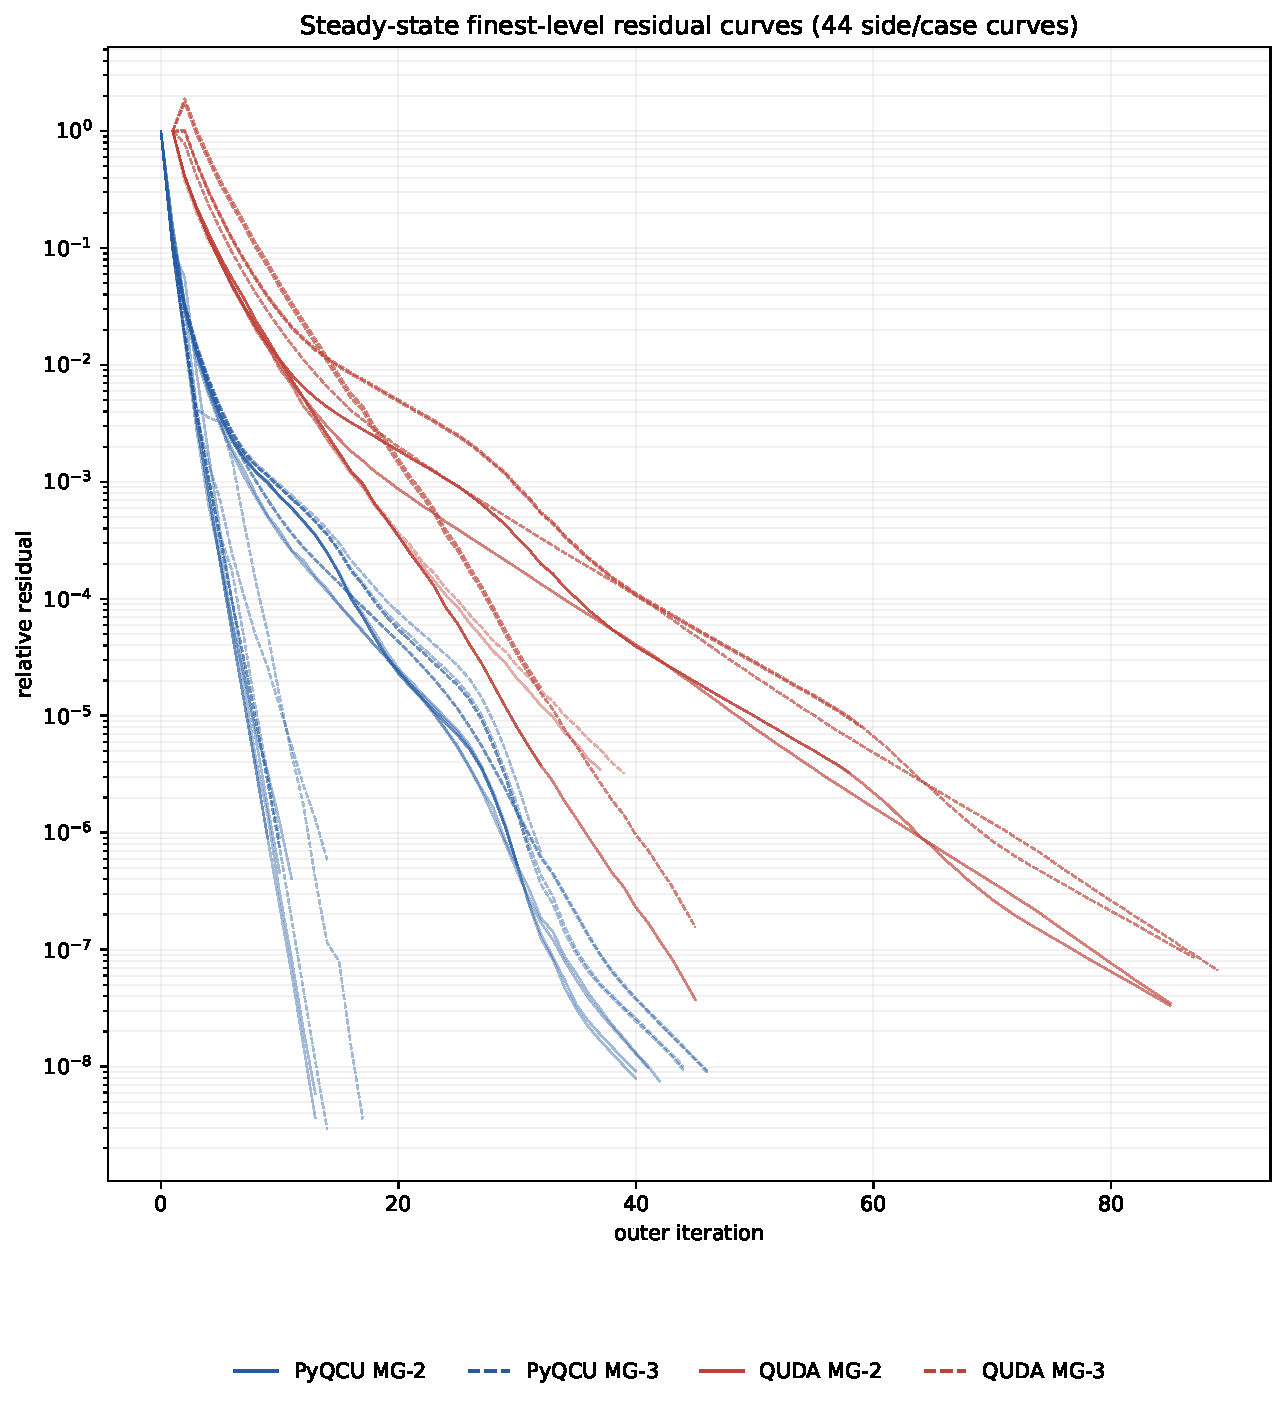
\includegraphics[width=0.94\linewidth,height=0.82\textheight,keepaspectratio]{mg_finest_residual.pdf}
\caption{最细层残差总览。44 条 side/case 曲线保留为细线，
PyQCU/QUDA 与 MG-2/MG-3 只用四个分组标签说明；图例固定放在绘图区
正下方，不覆盖坐标、曲线或刻度。}
\label{fig:finest-residual}
\end{figure}

两次递推标量的定义不同：PyQCU 主要记录 Arnoldi least-squares
estimate，QUDA 记录 GCR iterated residual。因此曲线用于观察下降趋势，
最终通过与否只由独立 full-operator true residual 判定。

\section{容量替代记录}

双 P100 的 $16\times32\times32\times48$ c64 请求项三次尝试均未同时
满足资源与时间门限：默认路径峰值约 15.9 GiB；
\code{PYQCU_MPI_OVERLAP=0} 约 14.8 GiB；extended CPU-staging
路径约 12.4 GiB，但 MG-2 setup 仍超过 570 s。该 6 个 combined 项
因此映射到已完整实测的 $16^4$ c64 对应项，并在
\path{capacity_substitutions.csv} 中显式标识。

\begin{table}[htbp]
\centering
\caption{容量替代项}
\small
\begin{tabularx}{\textwidth}{@{}L{0.27\textwidth}L{0.27\textwidth}L{0.13\textwidth}Y@{}}
\toprule
请求单元 & 有效单元 & 状态 & 原因 \\
\midrule
\path{p100__16x32x32x48__c64__l1__trace-off} &
\path{p100__16x16x16x16__c64__l1__trace-off} & substituted &
显存/时限 \\
\path{p100__16x32x32x48__c64__l1__trace-on} &
\path{p100__16x16x16x16__c64__l1__trace-on} & substituted &
显存/时限 \\
\path{p100__16x32x32x48__c64__l2__trace-off} &
\path{p100__16x16x16x16__c64__l2__trace-off} & substituted &
显存/时限 \\
\path{p100__16x32x32x48__c64__l2__trace-on} &
\path{p100__16x16x16x16__c64__l2__trace-on} & substituted &
显存/时限 \\
\path{p100__16x32x32x48__c64__l3__trace-off} &
\path{p100__16x16x16x16__c64__l3__trace-off} & substituted &
显存/时限 \\
\path{p100__16x32x32x48__c64__l3__trace-on} &
\path{p100__16x16x16x16__c64__l3__trace-on} & substituted &
显存/时限 \\
\bottomrule
\end{tabularx}
\end{table}

替代项只作为容量趋势证据，不与原大格公平加速比混合。完整中止记录见
\path{capacity_guard_events.json}。

\section{结论}

\begin{enumerate}
  \item 本版不改变 test27 的数值结论。66 个精确单元的全矩阵中位
        时间比为 1.0250，MG-2/3 合计 35/44 个单元优于 QUDA，
        BiCGStab 参考为 0/22。
  \item 绝对耗时使时间比的物理含义更清楚。例如 V100 c64
        $8^3\times16$ MG-3 trace-off 为 PyQCU 0.060 s、QUDA
        0.489 s，对应 $R=8.139$；而 V100 c128
        $16\times16\times32\times32$ MG-2 trace-off 为 PyQCU
        7.482 s、QUDA 4.041 s，对应 $R=0.540$。
  \item trace-on 的同步与诊断开销仍只用于阶段归因，正式性能结论
        使用 trace-off。
  \item 逐层重绘后，QUDA 的最粗层 solve 不再显示为零占位层。
        P100 c128 MG-3 的最粗层中位耗时为 PyQCU 14.781 s、
        QUDA 9.799 s；V100 c64 MG-3 则为 0.438 s 与 0.977 s，
        说明粗层优劣随设备、精度和层数显著变化。
  \item PyQCU/QUDA 最大真残差分别为 $7.40\times10^{-7}$ 与
        $7.97\times10^{-7}$，均通过 $5\times10^{-6}$ 门限；
        所有保留样本均低于 85\% 显存门限。
\end{enumerate}

\section{补充对照与复现}

\begin{figure}[htbp]
\centering
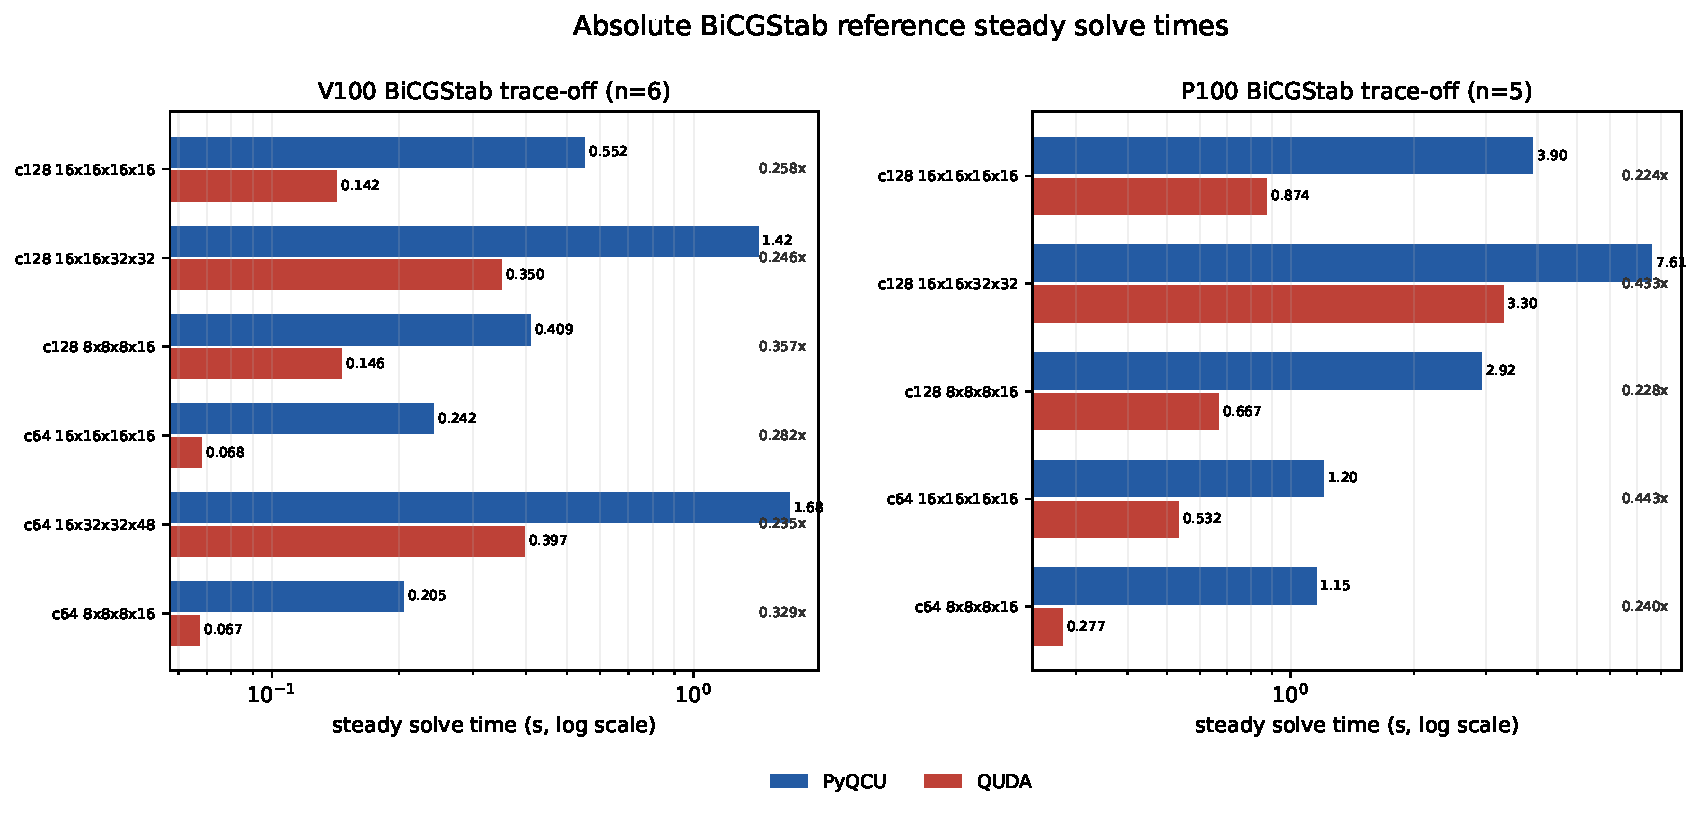
\includegraphics[width=0.98\linewidth,height=0.48\textheight,keepaspectratio]{mg_reference_runtime.pdf}
\caption{BiCGStab 参考的绝对 steady 耗时。该图用于明确区分
MultiGrid 与单层参考求解器，不把 BiCGStab 的时间比混入 MG 结论。}
\label{fig:reference-runtime}
\end{figure}

报告派生图与表格由
\path{pyqcu/testing/qcu/strict/quda_comparison/plot_mg_absolute_times.py}
从 test27 combined JSON 重建。输出目录为
\path{data/report_multigrid_comprehensive_20260929/report/}。

\begin{verbatim}
data/report_multigrid_comprehensive_20260928/final_protocol/
  combined/*.json
  units.csv
  stages.csv
  report/mg_matrix.csv
  report/mg_levels.csv
  report/mg_memory.csv

data/report_multigrid_comprehensive_20260929/report/
  unit_times.csv
  group_times.csv
  stage_times.csv
  stage_component_medians.csv
  coarsest_times.csv
  source_manifest.json
  mg_time_tradeoff.{pdf,svg}
  mg_runtime_traceoff.{pdf,svg}
  mg_reference_runtime.{pdf,svg}
  mg_stage_v100_mg2.{pdf,svg}
  mg_stage_v100_mg3.{pdf,svg}
  mg_stage_p100_mg2.{pdf,svg}
  mg_stage_p100_mg3.{pdf,svg}
  mg_finest_residual.{pdf,svg}
\end{verbatim}

原始采集、合并和审计入口仍为：
\begin{itemize}
  \item \path{pyqcu/testing/qcu/strict/quda_comparison/bench_mg_matrix_full.py}
  \item \path{pyqcu/testing/qcu/strict/quda_comparison/bench_strict_vs_quda.py}
  \item \path{pyqcu/testing/qcu/strict/quda_comparison/assemble_final_matrix.py}
  \item \path{pyqcu/testing/qcu/strict/quda_comparison/build_mg_report.py}
\end{itemize}

\end{document}
